\documentclass[11pt]{book}
\usepackage{amssymb,amsmath}
\usepackage{minitoc}
\usepackage{hyperref}
\usepackage{graphicx}
\usepackage{xcolor}


\title{Notes on BIOMEDE 211, or: \\ Circuits, Systems, \& Signals \\ in Biomedical Engineering}
\author{Barry Belmont}

\begin{document}
\frontmatter
\maketitle
\dominitoc
\tableofcontents


\newpage 
\section{How can I print off and use this document?}
Frankly, in just about any way that’s useful to you. I am going to try something here, where I will try to make more or less the entirety of the notes associated with the Winter 2019 semester of BIOMEDE 211, ”Circuits, Systems, and Signals in Biomedical Engineering”, to you, dear reader.\\
\\
Please don’t plagiarize this. If you were raised right, you ought to know what that is. If you’d like my judgment on any sort of action, my opinions can be laid bare.\\
\\
The first assignment I am giving you (worth 4\% of your grade and which must be completed by the end of the semester) is to figure out where this document is located online, download it, print it off, sign your name to it, and get it to me. If you know who I am, I would expect a competent engi- neer to find that without much to-do about it. Start with Google, go from there. Further, for those in the class, BIOMEDE 211, Winter 2019, you must join Github and make at least four substantive contributions to this repository. The term all you engineers (and lawyers) can’t wait to parse is “substantive” to which I will always enter a judgment which I deem final in this class, and I am ever in favor of beneficence over stricture. So, just help out the class in a way you think is helpful and watch those around you do the same. Failure to contribute to this living document by the end of the semester for those in this class will result in a loss of up to 4\% of one's total grade outright.

\newpage
\section{How can I contribute to GitHub?}
Follow these general steps to propose a change to this online document:
\begin{enumerate}
\item Create a GitHub account
\subitem This should be rather self-explanatory. Use your e-mail account and verify it to be able to edit. You should proceed with the following steps while logged onto your account.
\item Find Dr. Belmont's GitHub page and go to the biomede-211-w19 repository (``repo''). Then click on the biomede-211-w19.tex file.
\item Edit the file
\subitem You will find a small pencil icon on the right side of the page. Click on this to create your own branch (``forking''), and edit the file as you wish.
\item Propose file change
\subitem After making your changes, you should scroll to the bottom of the page, find the message box that says, 'Propose file change', and fill it out. The first line should say what you have updated and can be explained in the description.
\item Create pull request
\subitem After finishing your file, you will be brought to a page that displays what you have modified on the original document. Press the green `Create pull request' button to let Dr. Belmont know that you want to create a change. Once he has approved via his own GitHub account, your changes should now be in the updated master branch!
\end{enumerate}

\newpage



\section{Who comprises this class and how can they be reached?}
\subsection{The Captain at the helm}
Barry Belmont \\ Wednesdays 11:00 a.m. | 1:00 p.m., 2130 LBME \\ belmont@umich.edu \\
\subsection{The A-Team}
Annabelle St. Pierre \\ Wednesdays 5:00 p.m. | 6:30 p.m., UGLI basement \\ astpierr@umich.edu \\
\\
Alice Tracey \\ Wednesdays 4:00 p.m. | 5:00 p.m., UGLI basement \\ atracey@umich.edu \\

\subsection{You, yourselves}
In this class, we will be learning a lot from each other. You are encouraged to learn from one another. You are encouraged to talk to one another. You are are encouraged to share ideas and at times data. You are not encouraged and are hereby expressly forbidden to submit the work of another as your own. If you get help from others, you will put their name on it somewhere. Too much of this and you are committing plagiarism, not enough and you are committing fraud. Please be honest and let's all learn together.
\begin{enumerate}
	\item Kristian A.
	\item Matt A.
	\item Rayna B.
	\item Ellianna B.
	\item Megan B.
	\item Ashley B.
	\item Dawn C.
	\item Weihong C.
	\item Caila C.
	\item Jenna D.
	\item Sandra D.
	\item James G.
	\item Natalie H.
	\item Yazmin H.
	\item Felicia H.
	\item Isabel H.
	\item Danica J.
	\item Surabhi J.
	\item David K.
	\item Erica K.
	\item Eunjeong L.
	\item Annie L.
	\item Ian M.
	\item Madelynn M.
	\item Devak N.
	\item Likitha N.
	\item Bree P.
	\item Neelay P.
	\item Matei P.
	\item Shaunak P.
	\item Francesca Q.
	\item Raahul R.
	\item Abigail R.
	\item Alexander R.
	\item Andrew R.
	\item Elizabeth R.
	\item Kiana S.
	\item Ryan S.
	\item Sydney S.
	\item Hao S.
	\item Andrew S.
	\item Elijah S.
	\item Cara S.
	\item Aparna S.
	\item Alec S.
	\item Madison W.
	\item Jordyn W.
\end{enumerate}


\section{What is this class about?}
From the course catalog, ``Students learn circuits and linear systems concepts necessary for analysis and design of biomedical systems. Theory is motivated by examples from biomedical engineering. Topics covered include electrical circuit fundamentals, operational amplifiers, frequency response, electrical transients, impulse response, transfer functions and convolution, all motivated by circuit and biomedical examples. Elements of continuous time-domain and frequency-domain analytical techniques are developed.''

From your instructor's heart, "You’re going to learn the fundamental basis of electricity and its specific applicability to biomedical engineering, broadly. With this knowledge, you will have a command over a vaster swath of this world than most as you’ll know something important about how it works: namely, how human beings push electrons around the world to do some quite interesting things and how those electrons push back. This has relevance to a great many disparate situations: from the swelling of potential as your heart dances in your chest to nearly every source of light you’ve ever seen sans the sun (and even then...). All this to say, what we do here matters. And we’ll aim to do it well."

\section{When and where does this class meet?}
Tuesdays and Thursdays, 12:30 -- 2:30 p.m., 1006 DOW

\section{What is required for this class?}
\subsection{Writing materials}
A good pen and some sheets of paper ought to do.

\subsection{Access to the internet periodically}
A good bulk of our class’s administration will be done through Canvas. Check it regularly.

\subsection{A textbook of some kind}
Getting more than one perspective on a topic helps most people learn better. As such, in addition to the textbook which you are currently reading, I recommend consulting another electric circuits text. We have, in the past, used \textit{Fundamentals of Electric Circuits}, 6th edition, by Charles Alexander and Matthew Sadiku, which is also used by our EECS brothers and sisters. Digital or hardcopy is fine. As are older editions or equivalents.

\section{What determines the grade?}
\subsection{The abject material of the the thing}
Grades are determined essentially through three distinct types of assessment. 
\begin{itemize}
	\item The first and foremost of these are out-of-class based assignments (henceforth, ``homework''), individually worth 8 percent, and collectively worth 48 percent of the overall grade.
	\item The second and secondmost of these are three in-class based assignments (henceforth, ``glorious quizzes/exams'), which are worth 12, 12, and 20 percent of the overall grade, respectively. 
	\item The final type is the evaluation of a certain in-class/out-of-class \textit{je’nais se quoi} quality of the participatory student. ``Participation'' is something I take seriously in my classes and in this class will consist of (1) at least one in-class demonstration of your solutions to problems posed during the lecture period and (2) contribution to this specific document through the GitHub. Each of these forms of participation are worth 4 percent of the grade.
\end{itemize}

\subsection{The largely arbitrary, but nevertheless significant scale by which the grade will be measured by the instructors}
As this is my second time teaching this course, some calibration (on a per assignment and/or class- wide basis) may be required. That said, I plan on grading this class just as you might expect any other engineering class to do so against the following scale: \\
\\
\begin{center}
	A+ $\geq$ 97; A $\geq$ 94; A- $\geq$ 90; \\
	B+ $\geq$ 87; B $\geq$ 84; B- $\geq$ 80; \\
	C+ $\geq$ 77; C $\geq$ 74; C- $\geq$ 70; \\
	D $\geq$ 60; F $\geq$ 50
\end{center}

\subsection{The policy regarding missed chances, do overs, and dishonesty}
\begin{itemize}
	\item \textbf{If you will be absent} for some key assessment (a homework, an exam, participation), let the instructor know ahead of time and we can work something out.
	\item \textbf{If you feel the assessment of your work was wrong, misguided, or unfair}, let the instructor know immediately and specifically (within 48 hours of the assessment being returned) and we will work something out. 
	\item \textbf{If you insist at any point on swindling yourself out of an honest education}, please reconsider your decisions to do so (perhaps by discussing the matter with your instructor), otherwise this whole engineering thing for you is not going to work out. You are encouraged to read the Honor Code of the institution to which you are responsible.
\end{itemize}

\section{What are the objectives of this class?}
\begin{enumerate}
	\item To generate physical understanding of fundamental circuit and systems concepts.
	\item To relate classroom material to real-world applications including selected biomedical systems.
	\item To teach students basic circuit and linear systems including transient, frequency response, impulse response, and transfer functions.
	\item To introduce mathematical concepts necessary to accomplish the above including convolution, Laplace transforms, and Fourier transforms.
\end{enumerate}

\section{What are the outcomes I can expect of myself from this class?}
\begin{enumerate}
	\item Learn basic circuit and systems techniques necessary for understanding biomedical instrumentation systems, bioelectrical systems, and medical imaging systems.
	\item Develop an insight into systems analysis techniques motivated by development of electrical circuits concepts.
	\item Develop an insight into operational amplifier analysis and design techniques as motivated by a series of practical biomedical amplifier designs.
	\item Understand mathematical tools necessary for linear systems and circuit analysis/design.
\end{enumerate}



\mainmatter
\setcounter{page}{1}



\part{Circuits}



\chapter{I. Potential, current, energy, conservation}
01/10/2019
\minitoc



\section{What is electricity?}

\begin{enumerate}
	\item A form of energy resulting from the existence of charged particles 
	\item The physical phenomena arising from the existence, presence, and motion of charged particles
	\item Rather ill-defined in common vernacular – we will generally avoid its use
\end{enumerate}



\section{Charge}
 
\begin{enumerate}
	\item Charge is the property of matter that causes it to experience a force when placed in an electromagnetic field; measured in coulombs (C)
	\item 	Charges are found in nature in discrete, integral multiples of electronic charge: e  = -1.602 x $10^{-19}$ C (the charge of one electron)
	\item \textbf{How many electrons are needed to form one coulomb?} (What is the weight of all those electrons?) 
	\item One byte is eight bits. Bits are essentially a single electron stored in a transistor. \textbf{If we were to take all the electrons from one terabyte of well distributed information (equal number of ones and zeros), how many coulombs would we have?}
\end{enumerate}


\section{Current}
\begin{enumerate}
	\item The time rate of change of charge – charges (charged particles) in motion; measured in amperes; defined mathematically as
	\begin{equation}
	\label{i=dqdt}
		i := dq/dt
	\end{equation}
	where $i$ is current, $q$ is charge, and $t$ is time
	
	\item Conversely, the total charge transferred over time can be expressed as 
	\begin{equation}
	\label{q=it}
		Q := \int_{t_0}^{t}i dt
	\end{equation}

	\item 1 ampere is equal to 1 coulomb/second
	\item Direct current, ``DC'', is current that remains constant with time
	\item Alternating current, ``AC'', is current that varies sinusoidally with time
\end{enumerate}


\subsection{The directionality of current}
Ultimately, the direction in which we say "current" flows is largely arbitrary. As arbitrary as choosing one type of charge and calling it ``positive'' and another ``negative''. The reason it doesn't matter is that the only consequence of having chosen a ``wrong direction'' for the current in a given analysis is that we have to switch the sign of the value. Thus, 3 amps in one direction is \textit{the exact same thing }as -3 in the opposite direction.
\begin{enumerate}
	\item Thanks to Benjamin Franklin we say that current is 
	\subitem i.	\textbf{Positive in the direction in which positively charged particles flow} and 
	\subitem ii.	\textbf{Negative in the direction in which negatively charged particles}
	\subitem iii.	We also now know that current results primarily from the movement of negatively charged particles (electrons) and therefore our convention is “wrong” in one sense, though convenient and entrenched enough that we’re not liable to change it in our life time (besides, the math comes out the same, and the actual flow of electrons will only matter to us in a few special circumstances, diodes)
\end{enumerate}


\subsection{The at times deadly serious nature of current}
Much of the point of learning this material here is its eventual application by our hands or by the hands of those we work with. Before we put any of this stuff in our hands, we should probably know what is and is not safe.
\begin{enumerate}
	\item 1 mA, you will feel
	\item 10 mA, you will really feel
	\item 100 mA, you will likely die
	\item 1000 mA, you will definitely die
\end{enumerate}


\subsection{The ``speed'' of current}
A possible misconception is that the electrons inside a wire travels at the speed of light. The speed of current is actually relatively slow. If one were to imagine an electron starting at the wire next to a light switch in an average classroom, it would take a very long period of time for it to travel to the light itself. The light's immediate reaction to a switch is due to a ''hose effect''; the electrons inside the wire push other electrons in the direction opposite to the [conventional] current. This cascade of electrons is what happens close to the speed of light, not the electron movement itself.

\begin{enumerate}
	\item T\textbf{he \textit{signal} of electrical current (that is electromagnetic radiation) travels anywhere between about 50-99\% the speed of light} (dependent on a number of conditions) depending upon the material through which it travels (based on a “dielectric” behavior known as permittivity)
	\item \textbf{The drift velocity of electrons} within a copper wire is ~25 $\mu$m/s, so how does anything ever turn on?
	\item \textbf{The hose effect} - The electrons at the light switch will almost certainly never pass through a light bulb, but they will move around and bump into their neighbors which bump into their neighbors which bump into their neighbors, etc., until it causes the electrons nearest the light to pass through. This is how water at a spigot is able to push water at the end of a hose.
	\item \textbf{How current and drift veolcity related?} - Mathematically, it's represented as follow:
	\begin{equation}
		I = \frac{Q}{t} = \frac{neAd}{d/v_d}
	\end{equation}
	Imagine there is a cylindrical wire with length d and cross-sectional area A. Suppose there are n electrons per unit volume and each with a charge of e. Then in the whole cylinderical wire, the total charge is derived by multuplying the total volume Ad, the number of electron per unit volume n, and the elementary charge e. This is the numerator part of the story. On the denominator is the time component. Assume all electrons are moving in one direction and with drift veolcity. It would take t amount of time for the last electron to move a distance of d from one end to the other and exit the cylinderical wire. In fact, this is how we, in a microscopic sense, perceive the concept of current, which is defined by the total charge that passes through a single reference cross-section over a given amount of time. 
\end{enumerate}



\section{Potential (difference)}
\begin{enumerate}
	\item The amount of work needed to move a unit of (positive) charge from a reference point to another point [without producing an acceleration]).
	\item Potential is measured in ``volts'' and is often called ``voltage''. In this class we will endeavor to avoid such a term as it can be very confusing to talk about potential as if there were such a \textit{thing} as voltage.
	\item Defined as 
	\begin{equation}
		v:= \frac{dw}{dq}
	\end{equation}
	\item Potential describes the \textit{potential} to do something. Increasing the potential is akin to increasing the height of a cliff. The height does not \textit{do} anything other than increase what can be done on the drop. If potential is the cliff's height, charge would be pebbles you'd drop off the side, and current describes how fast those pebble fall.
	\item In this class, and for the vast vast majority of electrical engineering work, we care about the \textit{difference} in potential. One element held at 100 billion volts and another held at 100 billion + 1 volts has a \textit{potential difference} of 1 V, which is less than a single AA battery.
	\item Voltage can also be thought of as how badly the current "wants" to flow, while current is the actual flow of charges per second. Since charge flows but not the voltage, voltage can exist without current - a single charge induces a voltage. On the other hand, current can't exist without voltage since having a current means that charges are flowing, and if charges are flowing there is a potential difference across the charges. 
	\item Some typical voltages to be aware of
	\subitem \textbf{Consumer level batteries} (AA, AAA): 1.5 V (DC); 9 V (DC) 
	\subitem \textbf{Car batteries}: 12 V (DC)
	\subitem \textbf{The ``mains''} (levels provided by power companies to consumers): 110-120 V (AC) and 220-240 V (AC) in America
	\subitem \textbf{Power transmission lines}: 110-1200 kV (AC), transformers are used to step up and down the potential before used by consumers
\end{enumerate}



\section{Power}
\begin{enumerate}
	\item The time rate of expending or absorbing energy.
	\item Quantifies the rate of energy transfer.
	\item Mathematically:
	\begin{equation}
		p = \frac{dw}{dt} = \frac{dw}{dq}\cdot\frac{dq}{dt} = v\cdot i
	\end{equation}
	\item Measured in watts: 1 W = 1 $\frac{\text{J}}{\text{s}}$ = 1 $\frac{\text{N}\cdot \text{m}}{\text{s}}$ = 1 $\frac{\text{kg}\cdot \text{m}^2}{\text{s}^3}$ = 1 V $\cdot$ 1 A
	\item \textbf{Passive sign convention}: If current enters through the positive terminal of an element, $p = +vi$; if current enters through the negative terminal of an element, $p = -vi$.
\end{enumerate}



\section{Energy}
\begin{enumerate}
	\item The capacity to do work.
	\item Measured in joules.
	\item $E = \int\frac{dw}{dt}dt \rightarrow$ power x time
	\item J = $\frac{\text{kg}\cdot\text{m}^2}{\text{s}^2}$ = N $\cdot$ m = Pa $\cdot$ m$^3$ = W $\cdot$ s = C $\cdot$ V
\end{enumerate}



\section{Conservation}
Here, as elsewhere, things will be conserved. In electrical circuits there are two laws of conservation that will matter most for us:
\begin{enumerate}
	\item \textbf{The Conservation of Mass.} The conservation of mass means that no mass can be added to or removed from a circuit without being accounted for. Put differently, in a closed system (the type we will concern ourselves with here) no mass is added or removed.
	\subitem In electrical circuits, the mass we care the most about are the charges whipping around. Thus, for us, \textit{the amount of charge within a circuit must remain constant.}
	\item \textbf{The Conservation of Energy.} The conservation of energy means that no energy can be added to or removed from a circuit without being accounted for. Put differently, in a closed system (the type we will concern ourselves with here) no energy is added or removed.
	\subitem In electrical circuits, the energy we care the most about is the potential provided by sources and depleted by other elements in the circuits. Thus, for us, \textit{the sum of potentials within a circuit must equal zero.} 
\end{enumerate}

In evaluating circuits, the main focus of the first third of this class, it will be the application of these two conservative laws that will enable us to ``solve'' them. That is, by understanding (1) how energy is generated and used and (2) how charges move around in closed loops (``circuits'') we will be able to predict the behavior of the myriad electrical systems which may cross our paths.


 
\newpage



\section{Worksheet}

\subsection{Problem 1, constant charge through a cross-section}
How much charge passes through a cross-section of a conductor in 60 seconds if a DC current value is measured at 0.1 mA?
\textbf{Solution}


\subsection{Problem 2, arbitrary charge through a cross-section}
Determine the total charge entering a terminal between $t = 0$ seconds and $t = 10$ seconds if the current (in amps) passing through is
\begin{equation}
	i(t) = \frac{1}{\sqrt{5t+2}}. 
\end{equation} 
\textbf{Solution}


\subsection{Problem 3, a "tera"ble puzzle}
Approximately how much current is necessary to transmit one terabyte of information in an hour?
\textbf{Solution}


\subsection{Problem 4, power necessary to run a pacemaker}
A cardiac pacemaker will provide approximately 5,000 J of energy over 5 years. Determine the capacity of a 5 V lithium battery necessary to drive this pacing such that only 40\% of its energy is spent over that time.
\textbf{Solution}


\subsection{Problem 5, energy needed to excite a neuron}
A colleague of yours has been in their lab ginning up new neurons. You, as their resident electrical expert, are tasked with determining the energy consumed by the cell. If the current and voltage variations are found to be functions of time ($t \geq 0$)
\begin{eqnarray}
	i(t) = 3t \\
	v(t) = 10 e^{6t}
\end{eqnarray}
determine the energy consumed between 0 and 2 ms.
\textbf{Solution}


\subsection{Problem 6, a thump to the chest}
(a) A typical defibrillator delivers 200-1000 V in less than 10 ms. How much current is needed to deliver 120, 240, and 360 Joules?
\\
(b) A human heart ways about 300 grams. From approximately how high of a cliff would one have to drop a heart such that the impact was equivalent to the energy delivered to someone's chest from a defibrillator?
\textbf{Solution}



\chapter{An introduction: II. Circuit elements}
\minitoc
01/15/2019
\section{Active v. passive}
\begin{enumerate}
	\item Active elements are capable of generating energy while passive components cannot
	\item \textbf{Active}: generators, batteries, operational amplifiers, ``sources''
	\item \textbf{Passive}: resistors, capacitors, inductors, i.e., most circuit elements
\end{enumerate}

\section{Ohm's Law and what it means}

Ohm's Law is concerned with the relationship between voltage, or potential difference, and current across a conductor.  The potential difference across a conductor is proportional to the current flowing thorugh the conductor with the proportionality constant being denoted as R, or resistance.  This can be expressed as:

	\begin{equation}
	\label{V=iR}
		V := iR
	\end{equation}
	
This essentially states that the drop in potential across the conductor, or resistor, is equivalent to the current flowing through the conductor and its resistance.  When considering impedance, the equation can be modified to state:

	\begin{equation}
	\label{V=iZ}
		V := iZ
	\end{equation}

\section{Sources}
\begin{enumerate}
	\item \textbf{An ideal independent source} is an active element that provides a specified value of potential or current, regardless of other circuit elements.
	\subitem Batteries and power supplies may be approximated as ideal potential sources.
	\item \textbf{An ideal dependent (or controlled) source} is an active element in which the source quantity is controlled by another quantity (such as potential, current, temperature, measured resistance, etc.).
	\item \textbf{An ideal potential source} will produce any current required to ensure that the terminal voltage stated is satisfied.
	\item \textbf{An ideal current source} will produce any voltage required to ensure that the terminal current as stated is satisfied
	\item Symbols
	\subitem Voltage-controlled voltage source, VCVS
	\subitem Current-controlled voltage source, CCVS
	\subitem Voltage-controlled current source, VCCS
	\subitem Current-controlled current source, CCCS 
\end{enumerate}

\section{Resistors}
\textbf{Resistors} are electrical (circuit) elements that resist the flow of electric charge (current); passive two-terminal components that implement a defined/``constant'' resistance; meant to reduce current flow and change potential

\subsection{Resistance, $R$}
\begin{enumerate}
	\item \textbf{Resistance} is the physical property describing an element's ability to resist current and is most often represented by $R$
	\item Resistance is measured in ``ohms'', $\Omega$, which is equivalent to 1 V/A
	\item Resistance is one half of a broader physical phenomenon known as \textbf{``impedance''} - the property describing an element's ability to \textit{impede} current. Impedance is typically represented by $Z$, which we'll explore more thorough in a bit.
\end{enumerate}

\subsection{Resistivity, $\rho$}
\begin{enumerate}
	\item The resistance of an element (such as a resistor) depends on three things: 
	\subitem \textbf{Resistivity}, $\rho$, of the material comprising the element, which is the \textit{material}'s ability to resist the flow of charges; measured in ohm-meters
	\subitem \textbf{Length}, $l$, of the element; measured in meters
	\subitem \textbf{Area}, $A$, of the cross-section of the element; measured in m$^2$
	\subitem Such that $R = \rho\frac{l}{A}$
	\subsubitem What units are we left with?
	\subsubitem What are the effects of length and area?
	\item \textbf{Materials with low resistivity} are generally called (and treated as) ``conductors'' as they are able to more effectively \textit{conduct} the motion of electrical charges than materials with high resistivity
	\item \textbf{Materials with very high resistivity} are generally used as ``insulators'' as they prevent the flow of current through them and thus \textit{insulate} the current within prescribed bounds, such as with a copper wire with plastic wrapped around it.
\end{enumerate}

Here is a link to a video that further explains the concepts of resistivity and resistance: \url{<https://www.youtube.com/watch?v=4rsswT_Rv1M>}.

\subsection{Conductance}
\begin{enumerate}
	\item The inverse of resistance is conductance, $G$, which describes the ability of an element to conduct current
	\item Measured in Siemens
	\item Allows us express Ohm's law slightly differently, $i = Gv$, which says that the current generated through an element by a potential is directly proportional to some constant, namely conductance.
	\item The material specific property \textbf{conductivity}, $\sigma$ is measured in S/m
\end{enumerate}

\section{Capacitors}
\begin{enumerate}
	\item Passive two-terminal components that store energy in an electric field; introduces capacitance to a circuit.
	\item Can be thought of as two conductive plates sandwiching a ``dielectric'' material. Essentially it is two ``conductors'' separated by a ``non-conductive region''.
	\item When a capacitor is attached across a source, an electric field develops across the dielectric causing a net positive charge to collect on one conductor and a net negative charge to collect on the other.
	\item We can define the capacitance of an element mathematically as 
	\begin{equation}
		C = Q/V
	\end{equation}
	where $C$ is capacitance in farads, $Q$ is positive or negative charge on each conductor, and $V$ is the potential between them
	\item We can also represent capacitance by the voltage-based rate of charge accumulation: $C = dQ/dV$.
\end{enumerate}

\subsection{Its time varying behavior}
Unlike resistors, capacitors have a \textit{time-varying} element to that. That is, since $C = Q/V$, $V = Q/C$.

If we then recall Equation \ref{q=it}, we can write the time-dependent potential relationship of a capacitor
\begin{equation}
	V(t) = \frac{Q(t)}{C} = \frac{1}{C}\int_{t_0}^{t} i(\tau) d\tau + V(t_0)
\end{equation}

We can also recall\footnote{We could also take the derivative of the equation preceding this one and do a little rearrangement. As it turns out, these physical relationships are rather codified and thus can be gotten out by any number of means.} Equation \ref{i=dqdt}, and represent the time-dependent current relationship as
\begin{equation}
	I(t) = \frac{dQ(t)}{dt} = C\frac{dV(t)}{dt}
\end{equation}

\subsection{Charge accumulation}
\begin{enumerate}
	\item While charges accumulate on a capacitor, no current flows \textit{through} the capacitor.
	\item \textbf{Well, then why use them? After awhile won't the current just stop?} Yes, indeed it will -- in a DC circuit!
	\item The capacitor will become ``charged'' over time, eventually reaching the same potential as that established across it, e.g., by a source. Since potential only ever travels down potential gradients, if the capacitor and the source (say, a battery) are at the same potential, no current will flow.
	\item Thus, a fully charged capacitor will act as an ``open'' circuit, while an uncharged capacitor will act as a ``short'' circuit.
\end{enumerate}

\subsection{A simple example}
If we consider Ohm's law for a simple RC circuit (one in which a source, a resistor, and a capacitor are in series), we can describe the system by

\begin{align}
	V_0 &= v_{R}(t) + v_{C}(t) \\
	V_0 &= i(t)R + \frac{1}{C}\int_{t_0}^t i(\tau)d\tau
\end{align}
Taking the derivative of both sides:
\begin{align}
	0 &= R\frac{di(t)}{dt} + \frac{1}{C}i(t) \\
	0 &= RC\frac{di(t)}{dt} + i(t) \\
	i(t) &= \frac{V_0}{R}\cdot e^{-t/RC} \\
	v(t) &= V_0\left(1 - e^{-t/RC}\right) \\
	Q(t) &= C\cdot V_0\left(1 - e^{-t/RC}\right)
\end{align}


\section{Inductors}

\begin{enumerate}
	\item Passive two-terminal components that store energy in a magnetic field
	\item Can be thought of as an insulated wire wound into a coil around a core (which may either be filled with a material or left open to the environment)
	\item Behavior can be modeled as $L = \frac{\Phi}{I}$, where $L$ is the inductance, $\Phi$ is the magnetic flux generated by a current, $I$.
	\item By Faraday's law of induction, voltage induced by a change in magnetic flux through a circuit is
	\begin{equation}
		v = \frac{d\Phi}{dt}
	\end{equation}
	which we can rewrite as
	\begin{equation}
		v = \frac{d}{dt}(Li) = L\frac{di}{dt}
	\end{equation}
	\item In this class, at this level, and for most biomedical applications you're liable to experience in your tenure, you will not work extensively with inductors. However, you should be able to recall at least this much at a moment's notice to be able to ascertain a system's behavior.
\end{enumerate}




\section{Impedance}

\begin{enumerate}
	\item The measure of opposition a circuit element presents to a current when a potential is applied. (It is measured in ohms.)
	\item It is ``complex'' in two sense of the term. First, the actual phenomenon itself comprises complex numbers; that is, there is both a ``real'' and an ``imaginary'' component.
	\subitem \textbf{The real component} is known as resistance, $R$
	\subitem \textbf{The imaginary component} is known as reactance, $X$
	
	Impedance can be represented as a combination of either
	\subitem \textbf{Resistance and reactance}: $\mathbf{Z} = R + \jmath X$, where $\mathbf{Z}$ is impedance, $R$ is resistance, and $X$ is reactance, or
	\subitem \textbf{Magnitude and phase}: $\mathbf{Z} = |Z|e^{\jmath \theta}$, where $|Z|$ is the magnitude of the impedance vector, $\mathbf{Z}$, and $\theta$ is the phase of said vector (i.e., the delay between current and potential). Phase, $\theta$ is equivalent to $\tan^{-1}(X/R)$
	\item Impedance is also complex in the sense that it is complicated. The impedance of an object is a factor of many parameters including permittivity, geometry, quantum states, thermal stability, etc. Let us not view this sort of complexity as an impediment to our understanding of impedance.
	\item The inverse of impedance is \textbf{admittance}, $Y$, and comprises a real component, \textbf{conductance}, $G$, (which is the inverse of resistance) and an imaginary component, \textbf{susceptance}, $B$ (which is the inverse of reactance). (It is measured in Siemens.)
	\subitem $\mathbf{Y} = G + \jmath B$
\end{enumerate}

\subsection{A quick note on ``imaginary'' numbers}
The term ``imaginary'' is an unfortunate name for an excellent mathematical tool. All the imaginary operator -- in this class represented by $\jmath = \sqrt{-1}$ -- is is a type of number ``orthogonal'' to our ``real'' numbers. Imaginary numbers are no less ``real'' than real numbers. Unfortunately, they aren't necessarily the most intuitive to our little mammalian brains and thus we must be trained to work with them. However, as we will see in this class, they can be quite useful.

\section{Equivalent impedance}
\begin{enumerate}
	\item It will often be more convenient to think about the impedance which a component burdens a system with (or the conductance which it affords) rather than its resistance. \textbf{Therefore, we need to begin to think in terms of equivalent impedances as we start to evaluate circuits.}
	\item Recall Ohm's law 
	\subitem \textbf{Resistors}, $v = iR \qquad \qquad \rightarrow Z_{eq,R} = R$
	\subitem \textbf{Capacitors}, $v = \frac{1}{C}\int i dt \quad \rightarrow Z_{eq,C} = \frac{1}{\jmath \omega C}$
	\subitem \textbf{Inductors}, $v = L\frac{di}{dt} \quad \qquad \rightarrow\jmath \omega L$
	
	I want to plant a flag here for you to notice the relationship between the $\jmath \omega$ terms from the capacitor and inductor and the corresponding derivative and integral forms of current in the Ohm's law representation. This will become very important once we get into the Laplace and Fourier transforms.
	\item We must also recognize that few will be the circuits comprising but a single element. As such, we should know how to find the equivalent impedance of many elements.
\end{enumerate}

\subsection{Impedances in general}
\textbf{Series}
\begin{equation}
	\label{zeq,ser}
	Z_{eq,series} = Z_1 + Z_2 + Z_3 + ...
\end{equation}
\\
\textbf{Parallel}
\begin{equation}
	\label{zeq,par}
	\frac{1}{Z_{eq,parallel}} = \frac{1}{Z_1} + \frac{1}{Z_2} + \frac{1}{Z_3} + ...
\end{equation}
\\
\textbf{A special case to remember}. When dealing with only two elements:
\begin{equation}
	\label{zeq,two}
	Z_{eq} = \frac{Z_1\cdot Z_2}{Z_1 + Z_2}
\end{equation}

\subsection{Resistors}

\textbf{Series}
\begin{equation}
	\label{req,ser}
	R_{eq,series} = R_1 + R_2 + R_3 + ...
\end{equation}
\\
\textbf{Parallel}
\begin{equation}
	\label{req,par}
	\frac{1}{R_{eq,parallel}} = \frac{1}{R_1} + \frac{1}{R_2} + \frac{1}{R_3} + ...
\end{equation}


\subsection{Capacitors}
\textbf{Series}
\begin{equation}
	\frac{1}{C_{eq,series}} = \frac{1}{C_1} + \frac{1}{C_2} + \frac{1}{C_3} + ...
\end{equation}
\\
\textbf{Parallel}
\begin{equation}
	C_{eq,parallel} = C_1 + C_2 + C_3 + ...
\end{equation}

\subsection{Delta-Wye ($\Delta$-$Y$) transformations}
\textbf{Going from Delta to Wye}
\begin{align}
	Z_1 = \frac{Z_b Z_c}{Z_a+Z_b+Z_c} \\
	Z_2 = \frac{Z_a Z_c}{Z_a+Z_b+Z_c} \\
	Z_3 = \frac{Z_a Z_b}{Z_a+Z_b+Z_c}
\end{align}
\\
\textbf{Going from Wye to Delta}
\begin{align}
	Z_a = \frac{Z_1Z_2 + Z_2Z_3 + Z_1Z_3}{Z_1} \\
	Z_b = \frac{Z_1Z_2 + Z_2Z_3 + Z_1Z_3}{Z_2} \\
	Z_c = \frac{Z_1Z_2 + Z_2Z_3 + Z_1Z_3}{Z_3} \\
\end{align}

\subsection{A few examples}
\textbf{Example 1}
Find the equivalent resistance, if a resistor $R_1 = 10 \text{ k}\Omega$ is connected in parallel to $R_2 = 3.3 \text{ k}\Omega$.

\textit{Solution}. $R_{eq} = \frac{R_1 \cdot R_2}{R_1 + R_2} = \frac{(10)(3.3)}{10 + 3.3} = 2.48 \text{ k}\Omega$
\\
\\
\textbf{Example 2}
Find the equivalent resistance of three parallel-connected resistors of equal value. If $R = R_1 = R_2 = R_3 = 10 \text{ k}\Omega$, what's $R_{eq}$?

\textit{Solution}.
Recall, Equation \ref{req,par}
\begin{equation}
	\frac{1}{R_{eq}} = \frac{1}{R} + \frac{1}{R} + \frac{1}{R} \rightarrow 3R_{eq} = R \rightarrow R_{eq} = \frac{R}{3} \rightarrow R_{eq} = \frac{10k}{3} = 3.33 k\Omega
\end{equation}
\\
\\
\textbf{Example 3}
Four resistors are connected in parallel. $R_1 = 10 \text{ k}\Omega$, $R_2 = 1 \text{ k}\Omega$, $R_3 = 5 \text{ k}\Omega$, and $R_4 = 3 \text{ k}\Omega$. Calculate their equivalent resistance.
\begin{align}
	\frac{1}{R_{eq}} &= \frac{1}{R_1} + \frac{1}{R_2} + \frac{1}{R_3} + \frac{1}{R_4} \\
	\frac{1}{R_{eq}} &= \frac{1}{10k} + \frac{1}{1k} + \frac{1}{5k} + \frac{1}{3k} \\
	&= 612.3 \text{ }\Omega
\end{align}

\section{Grounds}
\begin{enumerate}
	\item A reference point in an electrical circuit from which potentials are measured
	\item A common return path within a circuit
\end{enumerate}


\section{Conductors}
\begin{enumerate}
	\item Allow from the transmission of electrical energy
	\item Serve to connect circuit elements
	\item Also known as wires and traces
	\item Within circuit schematics we must be mindful of ``junctions'' and ``jumps'' in conductors
\end{enumerate}


\section{Operational amplifiers ("Op-amps")}
\begin{enumerate}
	\item Active components that deliver the amplified difference between its inverting and non-inverting terminals
	\item Will be discussed at length in the next class and along with resistors, capacitors, and sources, will be among the primary circuit components we work with
	\item Allow us to model mathematical functions; any mathematical function that can be represented by a differential equation can be replicated with an op-amp
\end{enumerate}


\section{Diodes}
Two-terminal circuit elements that allow current to flow only in one direction

\section{Switches}
Make/break/change circuit paths (thereby diverting current or removing potential)

\begin{enumerate}
	\item Single pole, single throw, SPST
	\item Single pole, double throw, SPDT
	\item Double pole, single throw, DPST
	\item Double pole, double throw, DPDT
\end{enumerate}


\section{Transistors}


\section{Transformers}
\begin{enumerate}
	\item Transfer electrical energy between circuits using induction
	\item Allows for the effective transmission of power and the stepping up/down of potential
	\item Crucial for the transmission, distribution, and utilization of AC
\end{enumerate}

\newpage
\section{Worksheet}
\subsection{Problem 1, expressing power in ohms}
Utilizing Ohm's law, express units of power to include ohms.

\textbf{Solution}


\subsection{Problem 2, a couple toaster based problems}
A toaster draws 2 A at 120 V. What is its resistance?

\textbf{Solution}
\\
\\
How much current is drawn by a toaster with a resistance of 10 $\Omega$ at 110 V?

\textbf{Solution}

\subsection{Problem 3, currently conducting power}
In the circuit shown, calculate the current, $i$, the conductance, $G$, and the power, $p$.

\textbf{Solution}


\subsection{Problem 4, conductance of a sodium channel}
Conductance ($G$/$A$) of a sodium channel of a cell membrane at a specific time is 10 mS/cm$^{2}$. If the channel length as 100 nm, what is its conductivity?

\textbf{Solution}


\subsection{Problem 5, resistance of a simple tissue}
Determine the resistance of a homogenous and isotropic tissue with a cross-sectional area which can be described by the functions $y = 8 - x^2$ from $x = -2$ cm to $x = +2$ cm, a length of 10 cm (parallel to the z-axis), and a resistivity of 80 $\Omega$m.

\textbf{Solution}




\chapter{An introduction: III. Operational amplifiers}
01/17/2019 
\minitoc

\section{Some details}
\includegraphics[width=0.5\textwidth]{figures/op-amp1}
\\
\includegraphics[width=\textwidth]{figures/op-amp2}

\begin{enumerate}
	\item Behaves like a voltage-controlled voltage source
	\item They can amplify, sum, subtract, multiply, differentiate, integrate
	\item They are active circuit elements
	\item Though they have somewhat more complicated internal workings, we typically represent them in electrical circuits as a triangle with three (sometimes five) very important terminals:
	\subitem An inverting input (— sign, typically represented up top for convenience, but it need not be)
	\subitem A non-inverting input (+ sign, typically on bottom)
	\subitem An output
\end{enumerate}

\section{Some rules}
There are \textbf{three important features of ideal operational amplifiers} that we must understand thoroughly. These are things worth stamping in your brain.

\begin{enumerate}
	\item \textbf{Infinite open-loop gain.} The ``A'' of the gain is infinitely large such that any difference in voltages $V_1$ and $V_2$ causes an enormously large output voltage. As much as is being supplied. (The real value of gain in most operational amplifiers is between $10^{5}$ and $10^8$.)
	\item \textbf{Infinite input impedance.} Current cannot travel between the inverting and non-inverting terminals. (Really, the impedance is between $10^5$ and $10^13$ ohms and is often signal dependent.)
	\item \textbf{Zero output impedance.} There is no loss transmitting a voltage difference to the output. (Really is about 10-100 ohms and is chip dependent.)
\end{enumerate}

\section{Some conveniences}
\begin{enumerate}
	\item With infinite input impedance, no current can flow into or out of the terminals and hence $i_1$ and $i_2$ are equal to 0.
	\item Since no current flows across the terminals, the terminals are at equal potential. Hence ``$v_1 = v_2$''.
\end{enumerate}

Some extra facts with operational amplifiers are that they can be combined with a capacitors to create different filters. Adding a capacitor in series with the input resistor creates a "high-pass filter" amplifier, where it passes signals with frequency higher than a specific cutoff frequency and attenutates signals lower than the cutoff. Adding a capacitor in parallel with the feedback resistor creates a "low-pass filter" amplifier, where it passes signals with frequency lower than the cutoff and attenuates signals higher than it. The corner frequency for the cutoff may be caulcated with f=1/(2piRC). Having both capacitors would create a band-pass filter which attenuates signals lower than the lower cutoff and higher than the upper cutoff frequencies.

\newpage
\section{Some examples}

\subsection{Inverting amplifier}
We will apply the conservation of mass at this point to solve our equations.  This is among the simplest and most effective ways to add gain to a circuit. So much so that you will use it again and again and again in life and especially in labs

\includegraphics[width=0.5\textwidth]{figures/op-amp3}

We apply KCL at the node for v1
\begin{enumerate}
	\item I1 – i2 – i3 = 0
	\item I3 = 0
	\item I1 – i2 = 0
	\item I1 = i2
	\item I1 = (vi – v1)/R1
	\item I2 = (v1 - Vo)/Rf
	\item (vi – v1)/R1 = (v1 - Vo)/Rf
	\item V1 = V2 = 0
	\item Vi/R1 = -Vo/Rf
	\item Vo = -Rf/R1 * Vi
	\item R2/R1 is our gain, gain factor.
\end{enumerate}




\subsection{Non-inverting amplifier}
\includegraphics[width=0.5\textwidth]{figures/op-amp4}

Again, the name might imply what it does. It will amplify our input signal without inverting it.

We can again perform Nodal analysis.
\begin{enumerate}
	\item I1 – i2 – i3 = 0
	\item I3 = 0, since no current enters the non-inverting input
	\item I1 = i2
	\item (Vg – v2)/R1 = (v2 – Vo)/Rf
	\item –v2/R1 = (vi – Vo)/Rf
	\item Vo = (1 + Rf/R1) * Vi
\end{enumerate}



\subsection{Voltage follower}
\includegraphics[width=0.5\textwidth]{figures/op-amp5.png}

What if we didn’t have any resistors? $\rightarrow$ Vi = v2 = v1 = Vo $\rightarrow Vi = Vo$


\subsection{Summing amplifier}
\subsection{Differential amplifier (as homework)}



\chapter{Circuit analysis: I. Nodal analysis}
01/22/2019
\minitoc
\newpage
\section{Nodes and branches}
\begin{enumerate}
	\item \textbf{A branch} is any two-terminal element. (examples: Resistor, Capacitor, Wire, etc.) 
	\subitem \textit{\textbf{A branch} is any two-terminal element. What are some two-terminal elements we’ve learned?}
	\item \textbf{A node} (junction) is a point of connection between two or more branches. 
	\subitem \textit{\textbf{A node} is a point of connection between two or more branches. Often indicated by a dot. What else have we called a node? A junction.}
	\item A loop is \textbf{independent} if at least one branch is not part of any other independent loop. 
	\subitem \textit{\textbf{A loop} is any closed path within a circuit. A closed path formed by starting at a node, passing through a set of nodes, returning to the starting node without passing through any node more than once.}
\end{enumerate}

\subsection{The Seven Bridges of Konigsberg}
The Königsberg bridge problem asks if the seven bridges of the city of Königsberg (left figure; Kraitchik 1942), formerly in Germany but now known as Kaliningrad and part of Russia, over the river Preger can all be traversed in a single trip without doubling back, with the additional requirement that the trip ends in the same place it began.

\begin{center}
	\includegraphics{figures/04.konisberg.png}
\end{center}



\subsection{Independence}
A loop is independent if it contains at least one branch which is not a part of any other independent loop
\begin{enumerate}
	\item Each of the loops in the circuit at right are independent 
	\item Independent loops lend themselves to sets of equations to be solved!
\end{enumerate}

\subsection{Fundamental theorem of network topology}
Fundamental theorem of network topology states that the number of branches, $b$, must equal the sum of the independent loops, $l$ and nodes, $m$ minus one, that is
\begin{equation}
	b = l + n - 1
\end{equation}

With this fundamental theorem we can also “redefine”/”refine” our definition of series and parallel.
\begin{itemize}
	\item \textbf{Series} | two or more elements share a single node and thereby carry the same current
	\item \textbf{Parallel} | connected to the same two nodes and thereby have the same voltage across them (potential difference)
\end{itemize}

\begin{center}
	\includegraphics{figures/04.example1.png}
\end{center}

 
\newpage
\section{Kirchhoff's Laws}
I am not personally a fan named laws of nature, especially ones which are mere recapitulations of already perfectly good laws. Thus do we introduce Kirchhoff’s laws, known as 
\begin{itemize}
	\item Kirchhoff’s current law (``KCL'') 
	\item Kirchhoff’s voltage law (``KVL'')  
\end{itemize}
	
These are, as far as I’m concerned, mere restatements of \textit{the conservation of mass} and \textit{the conservation of energy}, respectively.


\subsection{Kirchhoff's Current Law}
\textbf{Kirchhoff's current law} states that any node (junction) in an electrical circuit, the sum of currents flowing into that node is equal to the sum of currents flowing out of that node.

\begin{itemize}
	\item Put differently, the algebraic sum of currents entering a node (or any closed boundary) is zero
	\item For those mathematically inclined among us, that is: $\sum_{x=1}^n i_x = 0$
	\item Another way this often gets stated is by saying that the algebraic sum of charges within a system cannot change and is thus sometimes referred to as ``the conservation of charge''.
	\item Well since all of our charge carriers are merely particles (electrons, protons, ions, etc.), this is just another layer over the top of the underlying law which is that mass cannot be created or destroyed.
	\item However, Kirchhoff's formulation of this law (conserving charge, mass) is useful in circuits as it gives us a great tool, being able to say that current going in is equal to current going out
	\item For the figure $i_1 + (-i_2) + i_3 + i_4 + (-i_5) = 0 \rightarrow i_1 +i_3 + i_4 = i_2 + i_5$
	\item KCL forms the basis of a technique we’ll spend the next couple of lectures on known as “nodal analysis” because we evaluate the current going into and coming out of nodes
\end{itemize}

\includegraphics{figures/04.node.png}
\includegraphics{figures/04.single-loop-kvl.png}

\subsection{Kirchhoff's Voltage Law}
Kirchhoff's voltage law states that the sum of electrical potential differences (voltage) around any closed network is zero
\begin{itemize}
	\item That is, for any closed path (loop), the sum of voltages is zero.
	\item Mathematically: $\sum_{m=1}^{M} v_m = 0$, where M is the number of voltage drops (caused by circuit elements) in the loop and vm is the $m$th voltage drop
	\item The sum of voltage rises = the sum of voltage drops
	\subitem $v_1 + (-v_2) + (-v_3) + v_4 + (-v_5) = 0$
	\subitem $v_1 + v_4 = v_2 +v_3 + v_5$
	
\end{itemize}

\subsection{A few examples}
\begin{enumerate}
	\item Simple 1 Vs – 1 R circuit; Vs = 10, R = 1 kohm, I = 0.01 A / 10 mA
	\item Simple 1 Vs – 2 R in series; Vs = 10, R = 1 kohm, I = 0.005 A / 5 mA
	\subitem \textit{What does KCL tell us? (Current is the same through  resistors). }
	\item Simple 10 mA source, 2 R (1 kohm) in parallel; What is the voltage?
	\subitem $i_1 + (-i_2) + (-i_3) = 0 ] \rightarrow i_1 = i_2 + i_3 \rightarrow i_1 = V/R_1 + V/R_2$ 
	\subitem $0.01 = V/1000 + V/1000 \rightarrow 0.01 = 2V/1000 \rightarrow 0.010/2*1000 = 5$ V
	\subitem \textit{Nodes are at the same voltage!}
	\item 10 mA up, 5 mA down, 2 R (1 kohm), Rl (500 ohm), all in parallel. What is the current through load Rl? [have someone come to the board and solve]
	\subitem When current sources are in parallel they add together 
	\item For the circuit shown below, use KCL to find the remaining branch currents
\end{enumerate}

\begin{center}
	\includegraphics{figures/04.example2.png}
\\
\includegraphics{figures/04.example3.png}

\end{center}

For Figure 2.13, you know to use KCL because the circuit contains two current sources. Ideal current sources will deliver whatever potential is necessary to obtain the desired current so we don't know how potential behaves through it.
If we look at node x and arbitrarily set $i_1$ as entering the node from the left, $i_2$ as exiting the node down the branch containing the resistor, and $i_3$ as entering the node from the right, then:
\subitem $i_1 - i_2 + i_3 = 0$
\subitem $2i_0 - i_0 + 5 = 0$
\subitem $i_0 = - 5 A $
The negative sign just means that the arbitrary direction we chose for our analysis is opposite of the actual direction of current flow

For Figure 2.77, start at a node with only one unknown current such as the upper right node.
\subitem $2 - i_4 - 4 = 0$
\subitem $i_4 = -2 A$
Repeat the process for remaining nodes
\subitem $7 + i_4 - i_3 = 0$
\subitem $i_3 = 7 + (-2) = 5 A$

\subitem $-i_2 - 3 - 7 = 0$
\subitem $i_2 = -10 A$

\subitem $i_1 + i_2 - 2 = 0$
\subitem $i_1 = 2 - (-10) = 12 A$

We could check our work by performing nodal analysis at the last node. However, it is not a necessary step as we have already found the desired unknowns.



\newpage
\section{Nodal analysis}
Nodal analysis | a general circuit analysis technique in which we try to determine the potential difference between nodes by applying KCL and KVL (in my experience, usually focusing a bit more on KCL)

Your textbook offers the following description of the technique which seems pretty good to me:
\begin{enumerate}
	\item Select a node as a reference. Assign voltages ($v_1, v_2, ..., v_{n-1}$) for the remaining n-1 nodes, all of which will be referenced with respect to the reference node.
	\item Apply KCL to each of the n-1 nonreference nodes. Use Ohm’s law to express the branch currents in terms of node voltages.
	\item Solve the resulting simultaneous equations (system of equations) for each unknown node voltage.
	\item It's as easy as that! But, well, actually, it can get a little hairy once you start to apply it in earnest.
\end{enumerate}


\subsection{The procedure}

\begin{center}
	\includegraphics{figures/04.typical-nodal-circuit.png}
\end{center}

\begin{enumerate}
	\item Begin by putting a reference, usually a ``ground''
	\subitem This ground can be one of two sorts: (1) \textbf{Earth ground} in which ultimately the whole earth is used as the reference point; or \textbf{Chassis ground} in which the case of the device in which the circuit is in will act as a reference as it will presumably be sufficiently large as to serve fine [this is also partly the reason why you can ``feel'' a MacBook charge up – its charger does not utilize a traditional ``earth ground''
	\subitem Either will suffice for our purposes here
	\item Next we label all the nodes.
	\subitem How many branches, nodes, and loops?
	\subitem 5 branches, 3 nodes, 3 loops. Satisfies our network condition. 
	\subitem You can give them any label you want, but I find working your way up from the ground in a clockwise manner and numbering them sequentially is a good habit to get into.
	\subitem Keep in mind that we typically set our reference node to have a voltage of 0. We can actually set it to be anything we’d like, but the math is often easier if we just make it 0.
	\item Then we apply KCL to each nonreference node in the circuit.
	\subitem At node 1, $IA - i1 - i2 - IB \rightarrow IA = IB + i1 + i2$
	\subitem At node 2, $IB + i2 - i3  IB + i2 = i3$
	\subitem Once we’ve got that, now it’s a matter of applying Ohm’s law. Thought typically written as V = iR, it is perhaps more helpful to write its full extension here and note that (Va – Vb) = iR
	\subsubitem $I = (Va - Vb)/R$
	\subitem Thus we can state
	\subsubitem $I1 = (v1 - v0)/R1 	\rightarrow I1 = G1(v1 - v0)$
	\subsubitem $I2 = (v1 - v2)/R2 \rightarrow I2 = G2(v1 - v2)$

\end{enumerate}





\section{Solving simultaneous equations}
\subsection{Cramer's Rule}
When given a system of linear equations, Cramer's Rule allows us to solve directly for the specific variable whose value we are looking for.

To use Cramer's Rule, the system of equations must satisfy two conditions:
\begin{enumerate}
	\item There must be the same number of equations as variables (the coefficient matrix must be a square).
	\item The determinant of the coefficient must be non-zero.
\end{enumerate}

Use the following steps to apply Cramer's Rule:
\begin{enumerate}
	\item Write the coefficient matrix of the system (call this matrix A). Make sure this is a square matrix; otherwise Cramer's Rule is not applicable.
	\item Compute the determinant of matrix A. Make sure that this value is non-zero; otherwise Cramer's Rule is not applicable here.
	\item Suppose the first variable of the system is x. Write the matrix Ax by placing the column of numbers to the right of the equals sign as the first column of Ax and using the non-x coefficients of matrix A as the remaining columns.
	\item The value of x is the determinant of Ax divided by the determinant of A.
	\item Repeat steps 3 and 4 to solve for any other variable as needed.
\end{enumerate}

Example implementing Cramer's Rule:
We will use the following system of equations to demonstrate how to use Cramer's Rule to solve for the value of x:

\begin{center}
x + y + z = 4
-x + 2y = 1
-y + z = 1
\end{center}

\begin{enumerate}
	\item Write the coefficient matrix A and check that it is a square matrix:
		\begin{center}
		\[
  		A=
  		\left[ {\begin{array}{ccc}
   		1 & 1 & 1\\
   		-1 & 2 & 0\\
   		0 & -1 & 1\\
  		\end{array} } \right]
		\]
		\end{center}
	\item Solve for the determinant of A. (|A| = 4). The determinant does not equal zero.
	\item Write the matrix Ax:
		\begin{center}
		\[
  		Ax=
  		\left[ {\begin{array}{ccc}
   		4 & 1 & 1\\
   		1 & 2 & 0\\
   		1 & -1 & 1\\
  		\end{array} } \right]
		\]
		\end{center}
	\item Solve for the determinant of Ax. (|Ax| = 4). 
	\item Solve for the value of x:
		\begin{center}
		x = $\frac{|Ax|}{|A|}$
		x = 1
		\end{center}
\end{enumerate}

Reference: Explanation and example inspired by "Solving System of Linear Equations: (lesson 4 of 5), Cramers Rule", MathPortal: https://www.mathportal.org/algebra/solving-system-of-linear-equations/cramers-rule.php. [Accessed 23 January, 2019].


\newpage

\section{Worksheet}
\subsection{Problem 1, KCL at a few nodes}
Use KCL to write equations at each node.
\begin{center}
	\includegraphics[width=0.5\textwidth]{figures/04.problem1.png}
\end{center}


\textbf{Solution}


\subsection{Problem 2, matrix notation}
Write the matrix form of the equations written above. 


\textbf{Solution}


\subsection{Problem 3, Cramer's rule}
Using Cramer’s rule on the matrix equations above, what are the results?


\textbf{Solution}


\subsection{Problem 4, Straight to the matrix}
Write the node-voltage equations to the circuit at right in the matrix form.
\begin{center}
	\includegraphics[width=0.5\textwidth]{figures/04.problem4.png}
\end{center}


\textbf{Solution}









\chapter{Circuit analysis: II. Mesh analysis}
01/24/2019
\minitoc
\newpage
\section{Clarifications on the homework}

\section{Mesh analysis}
\begin{itemize}
	\item A mesh is a loop which does not contain any other loops within it.
	\item ABEF and BCDE are meshes. ABCDEF is not.
	\item We apply KVL to find the mesh currents within a given circuit (this can be particularly helpful / convenient when dealing with parallel circuits).
\end{itemize}
\begin{center}
	\includegraphics{figures/05.mesh1.png}
\end{center}

\section{Steps of mesh analysis}
\begin{enumerate}
	\item \textbf{For each of your $n$ meshes assign a mesh current ($i_1$, $i_2$, ..., $i_n$).} You may draw them in any direction you want, but generally a nice clockwise direction will help with consistency.
	\item \textbf{Apply KVL to each of the n meshes.} Use Ohm’s law to express the voltages in terms of the mesh currents
	\item \textbf{Solve the resulting n simultaneous equations to get the mesh currents.}
\end{enumerate}

\subsection{Important condition for use}
Unlike nodal analysis, mesh analysis only works for ``planar” networks'' | that is one which can be written in two-dimensions without any branches.\footnote{Nonplanar networks can still be solved using nodal analysis.}

\section{An example}
\includegraphics[width=\textwidth]{figures/05.mesh2.png}

For the example seen above, we might at this point in our lives be tempted to solve the circuit with branch currents (the current that actually flows into and out of every branch. That is certainly a valid way by which to look at the problem. But now we're going to try another. We're going to try to understand ``mesh currents''.

Those branch currents can be formed into a pair of coupled equations
\begin{eqnarray}
	V_A - R_1 i_1 - R_3 i_3 = 0 \\
	V_B - R_2 i_2 - R_3 i_3 = 0 
\end{eqnarray}

We can also apply KCL at the node between the three resistors and recognize a third bounding equation: $i_1 + i_2 - i_3 = 0$. We can then solve these three equations through any number of means (substitution, elimination, etc.).

But mesh analysis allows us to model the situation more simply and often more efficiently.

We begin by defining two arbitrary mesh currents, $i_1$ and $i_2$. Then we apply KVL as we do a ``walk'' around the loop defined by the mesh current.
\begin{eqnarray}
	V_A - R_1i_1 - R_3(i_1 - i_2) = 0 \\
	-R_3(-i_1 +i_2) - R_2i_2 - V_B = 0
\end{eqnarray}
This given us two equations with two unknowns (the arbitrary mesh currents, $i_1$ and $i_2$, we defined).

\section{Another example}
\begin{center}
	\includegraphics{figures/05.mesh3.png}
\end{center}

For the circuit above, let's try to find the branch currents by performing mesh analysis (i.e., by. first finding the mesh currents).

\textbf{Solution.}

Obtain mesh current using KVL. For mesh 1:
\begin{equation}
	-15 + 5 i_1 + 10(i_1 - i_2) + 10 = 0
\end{equation}
which simplifies to 
\begin{equation}
	3i_1 - 2i_2 = 1
	\label{mesh1}
\end{equation}

For  mesh 2:
\begin{equation}
	6i_2 + 4 i_2 + 10(i_2 - i_1) - 10 = 0
\end{equation}
simplifying to
\begin{equation}
	i_1 = 2i_2 - 1
	\label{mesh2}
\end{equation}

\subsection{Solving it one way}
Perhaps the technique we'd most likely reach for if we knew nothing else about a situation is substitution. In this case, let's substitute equation \ref{mesh2} into equation \ref{mesh1}:
\begin{equation}
	6i_2 - 3 - 2i_2 = 1 \rightarrow i_2 = 1 \text{ A}
\end{equation}
And plugging that result back in
\begin{equation}
	i_1 = 2i_2 -1 = 2 - 1 = 1 \text{ A}
\end{equation}

And thus $I_3$ being equal to the difference in current between $i_1$ and $i_2$ is equal t zero.


\subsection{Solving it another}
Another way of doing this is by recognizing some of the techniques afforded to us by linear algebra. If we squint at the equations with a little bit of good brain wrinkling, we can see that 
\begin{equation}
	\begin{bmatrix}
		3 & -2 \\ -1 & 2
	\end{bmatrix}
	\begin{bmatrix}
		i_1 \\ i_2
	\end{bmatrix}
	=
	\begin{bmatrix}
		1 \\ 1
	\end{bmatrix}
\end{equation}
is just as valid of way of putting it as any other.

In this form we can use a few techniques to solve for the unknowns. One technique to be aware of given its deployability in those times in which you might need to write out your work is \textit{Cramer's rule}.

Cramer's rule says that 
\begin{eqnarray}
	i_1 = \frac{\Delta_1}{\Delta} \\
	i_2 = \frac{\Delta_2}{\Delta}
\end{eqnarray}
where
\begin{eqnarray}
	\Delta = 
	\begin{vmatrix}
		3 & -2 \\ -1 & 2
	\end{vmatrix}
	= (3)(2) - (-1)(-2) = 4 \\
	\Delta_1 = 
	\begin{vmatrix}
		1 & -2 \\ 1 & 2
	\end{vmatrix}
	= (1)(2) - (1)(-2) = 4 \\
	\Delta_2 = 
	\begin{vmatrix}
		3 & 1 \\ -1 & 1
	\end{vmatrix}
	= (3)(1) - (-1)(1) = 4 \\
\end{eqnarray}
Thus
\begin{eqnarray}
	i_1 = \frac{4}{4} = 1 \\
	i_2 = \frac{4}{4} = 1
\end{eqnarray}
which agrees with the results we obtained before.



\section{Yet another example}
\begin{center}
	\includegraphics{figures/05.mesh5.png}
\end{center}
Let's begin by defining the mesh currents (flowing clockwise around each mesh)

\begin{center}
	\textbf{Mesh 1}
\end{center}
\begin{equation}
	20(i_1 - i_3) + 10(i_1 - i_2) - 70 = 0
\end{equation}

\begin{center}
	\textbf{Mesh 2}
\end{center}
\begin{equation}
	10(i_2 - i1) + 12(i_2 - i_3) + 42 = 0
\end{equation}

\begin{center}
	\textbf{Mesh 3}
\end{center}
\begin{equation}
	20(i_3 - i_1) + 14i_3 + 12(i_3 - i_2 = 0
\end{equation}

Putting the equations into standard form:
\begin{eqnarray}
	30i_1 - 10i_2 - 20i_3 = 70 \\
	-10 i_2 +22 i_2 - 12 i_3 = -42 \\
	-20 i_1 - 12i_2 +46 i_3 = 0
\end{eqnarray}

In matrix notation that becomes:
\begin{equation}
	\begin{bmatrix}
		30 & -10 & -20 \\ -10 & 22 & -12 \\ -20 & -12 & 46
	\end{bmatrix}
	\begin{bmatrix}
		i_1 \\ i_2 \\ i_3
	\end{bmatrix}
	=
	\begin{bmatrix}
		70 \\ -42 \\ 0
	\end{bmatrix}
\end{equation}
While this can be solved any number of ways, in MATLAB one can simply write \texttt{I = R/V}, which should tell you something about what is ``going on'' mathematically in these operations.


\section{Writing mesh equations directly in matrix form}
Let's take a look at yet one more example.
\begin{center}
	\includegraphics{figures/05.mesh6.png}
\end{center}

We might, by now, begin to appreciate that one of our matrices is simply the resistances (impedances) of a mesh bundled up in one matrix, the currents bundled up in another, and the potentials bundled up in another, shown below.

\begin{equation}
	\begin{bmatrix}
		r_{11} & r_{12} & r_{13} \\
		r_{21} & r_{22} & r_{23} \\
		r_{31} & r_{32} & r_{33} \\
	\end{bmatrix}
	\begin{bmatrix}
		i_1 \\ i_2 \\ i_3
	\end{bmatrix}
	=
	\begin{bmatrix}
		v_1 \\ v_2 \\ v_3
	\end{bmatrix}
\end{equation}

To properly assemble these matrices there's just a few simple rules.


First, let's take a loop around each mesh and determine the equivalent impedance (of that mesh!)
\begin{itemize}
	\item \textbf{Mesh 1.} $R_2 + R_5 + R_6$
	\item \textbf{Mesh 2.} $R_2 + R_1 + R_3$
	\item \textbf{Mesh 3.} $R_3 + R_6 + R_5$
\end{itemize}

These will comprise values along the diagonal of the resistance (impedance) matrix ($r_{11}$. $r_{22}$, and $r_{33}$).

Next, let's look for elements that are shared among meshes
\begin{itemize}
	\item \textbf{Mesh 1 \& 2} share $R_2$, so $r_{21}$ and $r_{12}$ both become $-R_2$
	\item \textbf{Mesh 2 \& 3} share $R_3$, so $r_{23}$ and $r_{32}$ both become $-R_3$
	\item \textbf{Mesh 3 \& 1} share $R_5$, so $r_{13}$ and $r_{31}$ both become $-R_5$
\end{itemize}

Thus, our entire resistance matrix becomes

\begin{equation}
	\begin{bmatrix}
		r_{11} & r_{12} & r_{13} \\
		r_{21} & r_{22} & r_{23} \\
		r_{31} & r_{32} & r_{33} \\
	\end{bmatrix}
	=
	\begin{bmatrix}
		(R_2 + R_5 + R_6) & -R_2 & -R_5 \\
		-R_2 & (R_2 + R_1 + R_3) & -R_3 \\
		-R_5 & -R_3 & (R_3 + R_6 + R_5) \\
	\end{bmatrix}
\end{equation}

The matrix it buts up against is easy enough to construct, it is simply the mesh current of each mesh

\begin{equation}
	\begin{bmatrix}
		i_1 \\ i_2 \\ i_3
	\end{bmatrix}
	=
	\begin{bmatrix}
		i_1 \\ i_2 \\ i_3
	\end{bmatrix}
\end{equation}
	
And the potential matrix is the sum of sources in the direction of the mesh current

\begin{equation}
		\begin{bmatrix}
		v_1 \\ v_2 \\ v_3
	\end{bmatrix}
	=
	\begin{bmatrix}
		-v_A + v_B \\ v_A \\ -v_B
	\end{bmatrix}
\end{equation}

Giving rise to a final form which can be solved efficiently by any computation engine we put before us.
\begin{equation}
	\begin{bmatrix}
		(R_2 + R_5 + R_6) & -R_2 & -R_5 \\
		-R_2 & (R_2 + R_1 + R_3) & -R_3 \\
		-R_5 & -R_3 & (R_3 + R_6 + R_5) \\
	\end{bmatrix}
	\begin{bmatrix}
		i_1 \\ i_2 \\ i_3
	\end{bmatrix}
	=
	\begin{bmatrix}
		-v_A + v_B \\ v_A \\ -v_B
	\end{bmatrix}
\end{equation}



\chapter{Circuit analysis: III. Supernodes and supermeshes}
01/29/2019 – Lecture 6. 
\minitoc
\newpage
\section{A review of nodal and mesh analysis}
\subsection{Nodal analysis}
\begin{enumerate}
	\item Select a node as a reference. Assign voltages ($v_1$, $v_2$, ..., $v_{n-1}$) for the remaining n-1 nodes, all of which will be referenced with respect to the reference node.
	\item Apply KCL to each of the n-1 nonreference nodes. Use Ohm’s law to express the branch currents in terms of node voltages.
	\item Solve the resulting simultaneous equations (system of equations) for each unknown node voltage.
	\item (It’s as easy as that! But, well, actually, it can get a little hairy once you start to apply it in earnest.)
\end{enumerate}

\newpage
\section{Nodal analysis with an independent current source}
Let's begin by analyzing the following circuit.
\begin{center}
	\includegraphics{figures/06.example1.png}
\end{center}
\begin{enumerate}
	\item Begin by putting a reference, usually a ``ground''.
	\item Next we label all the nodes.
	\subitem How many branches, nodes, and loops? (5 branches, 3 nodes, 3 loops. Satisfies our network condition.)
	\subitem You can give them any label you want, but I find working your way up from the ground in a clockwise manner and numbering them sequentially is a good habit to get into.
	\subitem Keep in mind that we typically set our reference node to have a voltage of 0. We can actually set it to be anything we’d like, but the math is often easier if we just make it 0. 
	\item Then we apply KCL to each nonreference node in the circuit.
	\subitem At node 1, $IA - i1 - i2 - IB \rightarrow IA = IB + i1 + i2$
	\subitem At node 2, $IB + i2 - i3 - IB + i2 = i3$
	\subitem Once we’ve got that, now it’s a matter of applying Ohm’s law. Thought typically written as $V = iR$, it is perhaps more helpful to write its full extension here and note that $(Va – Vb) = iR$
	\item $I = (Va - Vb)/R$, Thus we can state
	\begin{itemize} 
		\item 	$I1 = (v1 - v0)/R1 	\rightarrow I1 = G1(v1 - v0)$
		\item $I2 = (v1 - v2)/R2	 \rightarrow I2 = G2(v1 - v2)$
		\item $I3 = (v2 - v0)/R3	 \rightarrow I3 = G3(v2 - v0)$
	\end{itemize}
	\item Now we can substitute these relationships into our previous equations
\end{enumerate}
\newpage

\section{A brief review of Cramer's rule}
\includegraphics[width =\textwidth]{figures/06.cramers.png}
\newpage

\section{Nodal analysis with voltage sources, \textbf{Supernodes}}
We often pick the reference node at one end of the source (and then we have one less unknown node voltage to solve.

Typical examples can be typically solved. Write current equations at nodes 1 and two.

\includegraphics{figures/06.example2.png}

\includegraphics{figures/06.example3.png}
If we try to write a current equation at node 1, we must include a term for current through the 10V source. We could assign an unknown, or...

Or we can create a ``supernode'' which we do by drawing a dashed line around several nodes, including the elements between them, and apply KCL more broadly

\begin{itemize}
	\item Recall that KCL says that the net current flowing through any closed surface must be equal to zero. Thus, we apply KCL to the supernode.
\end{itemize}
\begin{equation}
	\frac{v_1}{R_2} + \frac{}{v_1 - (-15)}{R_!} + \frac{v_2}{R_4} + \frac{v_2 = (-15)}{R_3} = 0
\end{equation}

Now you might be tempeted to write another current equation for the other super node, however, you’d find that the equation is equivalent to the one we just found. If we tried to solve by substitution, all the terms would drop out and we’d see that the matrix was singular (the determinant is 0, it won't tell you anything new. 

Instead we apply KVL, noting that $-v_1 - 10 + v_2 = 0$

Next, we find an expression for the controlling variable ix in terms of the node voltages. Notice that since in this case ix is the current flowing away from node 3 through R3, we can say ix = (v3 – v2)/R3.


\newpage

\section{Nodal analysis with controlled sources}
We approach it the same way, but we're mindful of the dependence
\begin{center}
	\includegraphics{figures/06.example4.png}
\end{center}


Write KCL equations at each node, including the current of the controlled source, just as if it were an ordinary current source

\begin{center}
	\includegraphics{figures/06.eqn1.png}
\end{center}

Next, we find an expression for the controlling variable ix in terms of the node voltages. Notice that since in this case ix is the current flowing away from node 3 through R3, we can say $ix = (v3 - v2)/R3$.
\begin{center}
	\includegraphics{figures/06.eqn2.png}
\end{center}

So long as only three of those variable are unknown (say the voltages), then it can be solved by whatever method you’d like.

\section{Mesh analysis with current sources}
\section{Mesh analysis with controlled sources, \textbf{Supermeshes}}



\chapter{Circuit analysis: IV. Circuit theorems}
02/05/2019 – Lecture 7. 
\minitoc
\newpage
\section{Circuit theorems}
Circuit theorems are ways of quickly describing, summarizing, analyzing circuit, based on some mathematical tricks, two of which we’ll review today: Thevenin and Norton equivalent circuits. 
\begin{itemize}
	\item \textbf{Thevenin} | taking a complex circuit seen between two terminals and representing it as a resistor in series with a voltage source
	\item \textbf{Norton} | taking a complex bit of circuitry between two terminals and representing it as a current source in parallel with a current source
\end{itemize}

\begin{enumerate}
	\item These only apply to ``linear circuits'' – that is, circuits made of (ideal) resistors, capacitors, inductors, op-amps, filters
	\item Non-linear elements include things like diodes, transistors, and some of the digital logic stuff we’ll get into later in the semester.
	\item It might pay us dividends for us to consider what we mean by linearity at this point in the semester as it will become very relevant in our up-coming analyses
\end{enumerate}

\section{Linearity}
Comprises two separate yet equally important properties

\begin{enumerate}
	\item Homogeneity | If the input (the excitation) is multiplied by a constant, the output (the response) is multiplied by the same constant
	\subitem $v = iR \rightarrow kv = kiR$
	\item Additivity | The response to a sum of excitations is equal to the responses to each individual excitation
	\subitem  $v_1 = i_1R; v_2 = i_2R; \rightarrow v = (i_1 + i_2)R = i_1R_1 +i_2R = v_1 + v_2$
\end{enumerate}

Much of what we will do in this class is linear and much in life, given sufficient approximating, can be considered linear. Such relationships are useful, if not always strictly true (recall that even wires have resistivities and resistors have frequency ranges)

Note that since power is $i^2R = v^2/R$, the relationship is a quadratic and thus our necessary assumptions of linearity are not applicable.


\section{Superposition}
\begin{itemize}
	\item Until now, we’ve been considering everything in a circuit always ``on'', but one of the things the linearity of the system allows us to do is to selectively turn on and off sources while we solve, so long as we sum them up in the end.
	\item This principle | \textbf{superposition} | states that the voltage (or current) through an element (in a linear circuit) is the algebraic sum of the voltages across (or current through) that element due to each independent source acting alone. 
	\item To apply the superposition principle
	\begin{enumerate}
		\item Turn off all independent source but one and find the output (voltage or current) due to that source [using any of the techniques you’ve previously learned]
		\item Do this for each independent source
		\item Find the total contribution [for any given element, or indeed for all of them] by adding all the contributions due to the independent sources
		\item (Leave in all dependent sources since they are controlled by circuit variables)
	\end{enumerate}
	\item To “turn off” a source:
	\subitem Voltage sources get replaced by a 0V source / a short circuit | \textbf{Turn voltage sources into wires}
	\subitem Current sources get replaced by a 0A source / an open circuit | \textbf{Cut current sources out}
\end{itemize}

\includegraphics[width=\textwidth]{figures/07.01.png} \\
\includegraphics[width=0.5\textwidth]{figures/07.02.png}


\section{Source transformation}
\textbf{Source transformation} is the process of replacing a voltage source $v_s$ in series with a resistor $R$ by a current source $i_s$ in parallel with a resistor $R$ or vice versa.
\includegraphics{figures/07.03.png}

\begin{itemize}
	\item We can prove these two are equivalent between a-b by short circuiting the two-terminals.
	\item If the sources are turned off, the resistance at terminal a-b are the same (R)
	\item If the terminals are shorted, current flowing from a to be is $i_{ab}$ = $Vs/R$ and $i_{ab}$ = $i_s$. Thus $Vs/R = i_s$
	\item You can also replace dependent sources this way, provided you’re careful, but we’ll skip that analysis here and I won’t encourage its use unless you personally feel comfortable with the material
\end{itemize}


\section{Thevenin equivalents}
\begin{itemize}
	\item A linear two-terminal circuit can be replaced by an equivalent circuit consisting of a voltage source, $V_{th}$, in series with a resistor, $R_{th}$
	\subitem $V_{th}$ is equal to open-circuit voltage of original network, $V_{th} = V_{oc}$
	\item If we were to short the connection across terminals a and b, we can see (as we did previously), that $i_{sc} = V_{th}/R_{th}$
	\subitem Thus the short-circuit current is equal to the current for the original circuit and the Thevenin equivalent.
	\item These two facts allow us to say something rather interesting, namely that the \textbf{Thevenin resistance} of a circuit is equal to the ratio of its open-circuit voltage and its short-circuit current. $R_{th} = V_{oc}/I_{sc}$
	\item Thus, \textbf{to determine the Thevenin equivalent circuit}, we start by analyzing the original network for its open-circuit voltage and its short circuit current. [A more robust derivation of this is shown in your book in chapter 4.7]
	\item \textbf{To find the thevenin equivalent resistance}:
	\subitem \textit{If there are \textbf{no} dependent sources}, turn off all independent sources in the network. $R_{th}$ is the input resistance to the network between the two terminals of interest
	\subitem \textit{If \textbf{there are} dependent sources}, still turn off all independent sources and apply superposition.
	\subsubitem Apply a voltage at the terminals and determine the resulting current. Then $R_{th}$ is the ratio of applied voltage and elicited current $v_o/i_o$
	\subsubitem Or apply a current and determine the resulting voltage. Use which ever you feel comfortable with.
\end{itemize}
\newpage

\subsection{An example}
Create thevenin equivalent circuit between a and b [$R_L$ is a potentiometer and thus its value can change. We want to simplify our understanding of how all the complex stuff before it will act.]

\includegraphics{figures/07.04.png}

\begin{enumerate}
	\item Start by turning off the independent sources (32 V and 2 A), replacing them with a short- and an open-circuit respectively
	\item This will yield our resistance as a 4 || 12 + 1 = (4*12)/16 + 1 = 4 ohms
	\item Next, identify what our $V_{Th}$ would be
	\item To find $V_{Th}$ we can apply mesh analysis
	\begin{eqnarray}
		32 – 4i1 -12i1 + 12i2 = 0 \\ 
		i2 = 2 \\ 
		i1 = 0.5 A \\ 
	\end{eqnarray} 
	then plug it in for the voltage across the 12 ohm 
	\begin{equation}
		V_{th} = 1_2(i_1-i_1) = 30
	\end{equation}
	\item Or could use nodal analysis
	\begin{equation}
		(32 – V_{th})/4 + 2 = V_{Th}/12 \rightarrow V_{Th} = 30 
	\end{equation} 
\end{enumerate}

\newpage

\section{Norton equivalents}
\begin{itemize}
	\item A linear two-terminal circuit can be replaced by an equivalent circuit comprising a current source, $I_N$ in parallel with a resistor $R_N$
	\subitem $I_N$ is equal to the short-circuit current through the terminals
	\item To find the Norton equivalent resistance, we start the same way we did for $R_Th$ | that is, short our voltage sources, open our current sources and find the resistance.
	\subitem Well then this should suggest to us that $R_N$ is equal to $R_Th$, and indeed they are equal.
	\item The Norton current, $I_N$, is equal to the short-circuit current. 
	\subitem So we merely find the current that would travel through the short 
\end{itemize}

\subsection{An example}
\includegraphics{figures/07.05.png}
\begin{enumerate}
	\item We begin by zeroing all of our independent sources 
	\subitem $R_N = 5 || (8 +4 +8 [+0]) = 5||20 = (5*20)/(5+20) = 4$ ohms
	\item We can apply mesh analysis to find $I_N$
	\subitem We can ignore the 5-ohm resistor as its in parallel with a short and current will always seek the path of least resistance.
	\subsubitem Recall our bioimpedance example where with increasing frequency caused the current to flow down a different branch, because with greater frequency the capacitor went from acting like an open circuit (at low frequencies) to a short circuit (at high frequencies), thus bypassing the other branch altogether.
	\begin{eqnarray}
		I_1 = 2  \\
		I_2 = 12 – 4i_2 +4i_1 – 8i_2 – 8 i_2 \rightarrow 4(2) – 20(i_2) = -12 \\ 
		I_2 = 1 = i_{sc} = I_N
	\end{eqnarray}
	\item Alternatively, we could have found the Thevinin voltage [meshing it up]
	\begin{eqnarray}
		i3 = 2 \\
		12 -4(i4) + 4(i1) – 8(i4) -5(i4) – 8(i4) \rightarrow 4(2) – 25(i4) = -12 \\
		I4 = 0.8 A
	\end{eqnarray}
	\subitem Since we know 0.8 A goes through the 5 ohm resistor, and since we know that that 5 ohm resistor experiences the same voltage drop as the open circuit, we simple multiple 5*0.8 to give us, 4 V
	\item Well since we know $R_N = R_Th$ is 4 and $V_Th$ is 4: $I_N = V_Th/R_Th = 1 A$
	\item Thus Norton and Thevenin circuits are two sides of the same “source transformation” coin
\end{enumerate}

\newpage

\section{Equivalents with dependents}
When we’ve got a dependent source, we can’t just remove the sources and combine impedances. Instead, we’ve got to analyze the circuit to find the open-circuit voltage and the short-circuit current (and indeed such an approach will work in all cases, it’s just a little bit more work on our parts)

\includegraphics[width=0.9\textwidth]{figures/07.06.png}

\begin{itemize}
	\item I’m personally a fan of finding the Thevenin open voltage because it just clicks with my brain a little better, but if you like the Norton short-circuit current, feel to take that approach
	\item So I apply nodal analysis
	\begin{eqnarray}
		I_x + 2i_x – V_{oc}/10 = 0 \rightarrow 3i_x = V_{oc}/10 \\
		\text{Next we write an expression for our controlling variable, ix} \\
		10 – V_{oc} = i_x(5) \rightarrow ix = (10 – V_{oc})/5 \\
		\text{We can substitute this into our previous equation} \\
		3*(10-V_{oc})/5 = Voc/10 \rightarrow \mathbf{V_{oc} = V_{Th} = 8.57 }
	\end{eqnarray}
	\item Now we can consider the short-circuit conditions.
	\begin{eqnarray}
		I_x + 2i_x i_{sc} = 0 \rightarrow 3i_x = i_{sc} \\
		I_x = 10/5 = 2 \rightarrow \mathbf{I_{sc} = 3i_x = I_N = 6} 
	\end{eqnarray}
	\item From this, we can take the ratio of the open circuit voltage and the short circuit current and find the equivalent resistance of the network via Ohm's law: 8.57 V / 6 A = 1.43 ohms
\end{itemize}

\section{A step-by-step procedure}
\begin{enumerate}
	\item Perform two of these:
	\subitem Determine the open-circuit voltage $V_t = v_{oc}$
	\subitem Determine the short-circuit current $I_n = i_{sc}$
	\subitem Zero the independent sources and find the Thevenin resistance $R_t$ looking back into the terminals. Do not zero dependent sources
	\item Use the equations $V_t = R_tIn$ to compute the remaining value
	\item The Thevenin equivalent consists of a voltage source $V_t$ in series with $R_t$
	\item The Norton equivalent consists of a current source $I_n$ in parallel with $R_t$
\end{enumerate}


\chapter{A review of the material so far}
02/07/2019 

\section{A set of exercises in preparation of the first Glorifed Quiz}

\begin{enumerate}
	\item Find the equivalent resistance of the following [``+'' means ``in series with'', ``$\vert\vert$'' means ``in parallel with'']:
	\subitem a.	R1 + R2$\vert\vert$(R3 + R4)
	\subitem b.	(R1 + R2)$\vert\vert$(R3 + R4)
	\subitem c.	R1 + (R2 + R3$\vert\vert$(R4 + R5)||R6)
	\subitem d.	(R1$\vert\vert$R2$\vert\vert$R3)$\vert\vert$(R4$\vert\vert$R5$\vert\vert$R6)||(R7 + R8$\vert\vert$R9)
	\item To use superposition, one must turn off sources. A voltage source is replaced by what? A current source is replaced by what?
	\item A 5 µF capacitor has accumulated a total charge of 1250 µC. What is the voltage across the capacitor?
	\item Name each of the four types of dependent power sources and explain their functioning a bit beyond their name.
	\item The unit of current is the ampere, A. What are some equivalent units (for instance, what is its relationship to charge)?
	\item Does potential change instantaneously over the terminals of a capacitor?
	\item An RC circuit (in which ``R + C'', seen below) has a time constant, $\tau = RC$. Prove the following at a time $t_0$ when the switch is thrown to complete the circuit.
	
	\begin{center}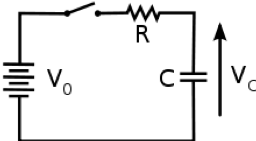
\includegraphics{figures/q1.01.png}\end{center}
	
	\subitem a. $I(t) = \frac{V_0}{R}\cdot e^{-t/\tau}$
	\subitem b. $V(t) = V_0\left(1-e^{-t/\tau}\right)$
	\subitem c. $Q(t) = C\cdot V_0\left(1-e^{-t/\tau}\right)$
	\item What is the difference between active and passive circuit elements?
	\item What can an ideal current source do what a real one cannot?
	\item What can ideal voltage source do what a real one cannot?
	\item Draw the symbol for a polarized capacitor.
	\item Draw the symbol for a potentiometer.
	\item Draw an op-amp, label its terminals, and explain what each does.
	\item What’s another name for a conductor?
	\item Which way does current run in a diode?
	\item Describe what Ohm’s law tells us in your own words.
	\item What is conductance? State Ohm’s law using conductance. What does it tell us about eh current passing through conductive materials?
	\item What is the equation for resistance in terms of resistivity? If resistivity goes up, what happens to resistance? If the cross-sectional areas decreases, what results? If a resistor keeps the exact same cross-sectional area over a length L, yet we contorted it into a very weird shape (say a balloon-animal poodle), will its resistance remain the same according to the aforementioned equation. Does that agree with your intuition?
	\item A capacitor has a time variance of current according to the follow formulation $I(t) = \frac{dQ(t)}{dt} = C\frac{dV(t)}{dt}$. That might be useful to know. See if you can prove that relationship to yourself knowing that C = Q/V.
	\item What is an inductor and how does it work?
	\item What is impedance? What is impeded? What does the impeding?
	\item What is the real and imaginary component of impedance.	
	\item How would I represent impedance by a magnitude and phase?
	\item 	What is impedance’s inverse? What are its real and imaginary components?	
	\item What is the impedance of a resistor, capacitor, and inductor?
	\item Find the equivalent impedance of the following, being sure to remove imaginary numbers from the denominator [``+'' means ``in series with'', ``$\vert\vert$'' means ``in parallel with'']:
	\subitem a.	Z1$\vert\vert$(Z2 + Z3)
	\subitem b.	(R1 + C1)$\vert\vert$C2$\vert\vert$(R2 + R3 + C3)
	\subitem c.	(R1 + L1)$\vert\vert$(C1 + L1)$\vert\vert$(C1 + R1)
	\item Convert a Wye circuit, with all R = 10 ohms, to a Delta circuit.
	\item Find the equivalent impedance of a Delta circuit of capacitors.	
	\item Given the following map, can you plan a parade rate that crosses each bridge exactly once? Why or why not?
	
	\begin{center}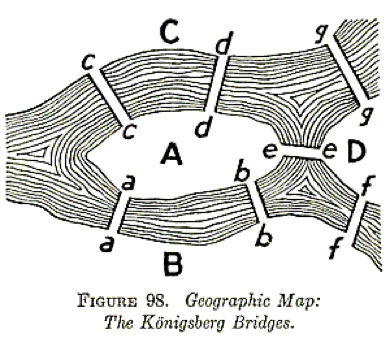
\includegraphics{figures/q1.02.png}\end{center} 
	
	\item 32.	Prove the fundamental theorem of network topology given any circuit (for instance, those aforementioned).
	\item Kirchhoff’s current law is a mere recitation of what other law of physics?
	\item Kirchhoff’s voltage law is a mere recitation of what other law of physics?
	\item When do we most use KCL? When do we must use KVL? Which do you prefer in general and why?
	\item Draw a complicated circuit (at least four branches) and solve for the current going through each component.
	\item Analyze the aforementioned complicated circuit using nodal analysis. Analyze said circuit with mesh analysis. Prove the validity of the fundamental theorem of network topology using said circuit.
	\item What is the difference between earth ground and chassis ground?
	\item Draw a circuit using each of the following, R1 = 10 ohms, R2 = 20 ohms, R3 = 30 ohms, R4 = 40 ohms, V1 = 20 V, V2 = 10 V, and I1 = 2 A. Solve using nodal analysis if you can (do you need to make a supernode?). Solve using mesh analysis if you can (do you need to make a supermesh?).
	\item Can you imagine modeling some actions in terms of circuits? For instance, if you were asked to model an equivalent circuit based on the operations of a shop floor, could you do it? If you were asked to model some aspect of physiology could you? The resistance of blood to flow? The capacitance of the lungs? The duration of our blinks?
	\item What is Cramer’s rule and how do we use it?
	\item Draw a circuit with at least five resistors and two current sources. Put that circuit into matrix formation for nodal voltages from inspection alone. What values should be along the diagonal, what values should be on the off-diagonal?
	\item To solve the above circuit in MATLAB, what would you type in?
	\item For any circuit stated previously, add a voltage source to one of the branches and solve using nodal analysis. What new technique did you need to employ and why did you need to? What does that technique do to our matrix?
	\item To any previously mentioned circuit, add a dependent current source and let it be dependent on the current going through R1. How does this change your nodal voltages?
	\item Given a jolt of 240 J from an AED, provide an energy equivalent. For example, how many little soft kitten jumps on the chest (1 kg, 5cm) is it equivalent to? It would be like falling from a height of how much? [Hint: the ground comes up at you.]
	\item A hospital consumes 500 kW in 60 seconds. How many people running on treadmills would it take to power it for a minute?
	\item A nurse starts their shift turning on medical doohickey that consumes 50 W at 220 V. How many electrons’ worth of charge pass through the doohickey before the nurse turns it off at the end of their shift, 10 hours later?
	\item Explain how mesh analysis works.
	\item Draw a mesh circuit with at least 6 unique elements. Analyze it.
	\item Draw another mesh circuit with at least four loops. Analyze it.
	\item For the two above-mentioned mesh circuits, put them directly into matrix form. What values go along the diagonal? What values go on the off-diagonals?
	\item For one of the mesh circuits you drew in either, add a dependent current source and solve using mesh analysis.
	\item How do we measure current and potential using actual ammeters and voltmeters? Why must we “break” the circuit to measure current? How do we measure potential across an element?
	\item Say, in as much detail as you can muster, what you believe the Thevenin circuit theorem is about.
	\item Say, in as much detail as you can muster, what you believe the Norton circuit theorem is about.
	\item Changing a potential source to a current source is an example of what technique to analyze circuits?
	\item What are two attributes necessary for things to be ``linear''?
	\item What is superposition and how do we use it to analyze a circuit?
	\item How do you turn off a voltage source in a circuit diagram? How do you turn off a current source?
	\item To one of the above dozen or so circuits you have drawn, find the Thevenin equivalent.
	\item To one of the above dozen or so circuits you have drawn, find the Norton equivalent.
	\item To the Thevenin in 62, convert it to its Norton equivalent. To the Norton in 63, convert it to its Thevenin equivalent.\
	\item What is an open circuit? What is a short circuit? How are they relevant to Thevenin and Norton equivalents?
	\item Draw an LM741 and label all 8 pins.
	\item What is an operational amplifier? What does it behave like? What can it do for us? How are they different from resistors, capacitors, and their ilk?
	\item What are the three key features we need to know to analyze op-amp circuits?
	\item Draw an inverting amplifier with R1 = 20 ohms, and R2 = 100 ohms. What is the gain on the input signal?
	\item Draw an inverting amplifier with Z1 = R1 = (Ra$\vert\vert$Rb) and Z2 = R2 = (Rc + Rb). Solve for the output voltage in terms of the input voltage.
	\item Draw a non-inverting amplifier with R1 = 100 kohms and R2 = 100 kohms.
	\item Draw the two circuits you drew above in series with one another. What is the output?
	\item What is a voltage follower and why is it important?
	\item If it’s so important you should be able to draw one and analyze its operation! Let’s do that. Draw a voltage follower and demonstrate its behavior in as much detail as you would need to convince another engineer you know what you’re talking about.
	\item Why might we want to use a voltage follower with an electrocardiogram?
	\item What is a summing amplifier?
	\item A summing amplifier can actually act as a logic converter is set up right. Can you imagine using a set of summing amplifiers to determine a winner in a simple tic-tac-toe game in which button presses turned on new voltage sources? Briefly describe how you could determine a winner.
	\item If I have a summing amplifier in which V1 = 10 V, R1 = 10 ohms, V2 = –10 V, R2 = 10 ohms, and Rf = 20 ohms, what is my output voltage?
	\item What is a differential amplifier and why is it important?
	\item Draw a differential amplifier. Analyze said differential amplifier. What is the output voltage in terms of the input voltage?
	\item What is a transfer function?
	\item You know how to go from a triangle (Delta) to a y (Wye) circuit for equivalence. How would you find the equivalent of going from a square to a cross?
	\item 	Draw a blood vessel. Find the electrical equivalent across the vessel and through the vessel.
	\item Draw the meanest circuit you think I’d ever give you on an exam. Then add a voltage dependent voltage source to one branch of it (its dependence rests on you). Solve it using nodal analysis, mesh analysis, superposition, and just plain looking at it.
\end{enumerate}



\chapter*{A Glorified Quiz I}
Given on February 12, 2019. All problems worth 10 points. Do not spend an inordinate amount of time on any given problem. Try your best.
\minitoc
\newpage

\section{Problem 1 on basic impedance}

Find the equivalent impedance of the following (``+'' means ``in series with'' and ``$\vert\vert$'' means ``in parallel with'') being sure that you end up with no imaginary terms in denominators. It may be helpful to draw these circuits as you understand them.
\begin{enumerate}
	\item 
	\item 
	\item 
\end{enumerate}


\section{Problem 2 on basic knowledge}
\begin{enumerate}
	\item 
	\item 
	\item 
	\item 
	\item 
\end{enumerate}

\section{Problem 3 on current and potential}
A current, $i(t)$, enters a device, causing a potential drop, $v(t)$. The current and the potential can be described mathematically as

\begin{equation*}
	i(t) = \begin{cases} 
      0 \text{ A}, & t< 0\\
      f(t) \text{ mA}, & t \geq0 \\
   \end{cases}
\end{equation*}
\begin{equation*}
	v(t) = \begin{cases} 
      0 \text{ V}, & t< 0\\
      g(t) \text{ V}, & t \geq0 \\
   \end{cases}
\end{equation*}

\begin{enumerate}
	\item 
	\item 
	\item 
\end{enumerate}

\newpage

\section{Problem 4 on transresistance amplification or bioamplification}
There are at least two kinds of current-to-voltage converters (also known as \textit{transresistance amplifiers)}.

\section{Problem 5 on equivalent impedance}
Choose one of the following (or do both for bonus points).
\begin{enumerate}
	\item Determine the equivalent impedance seen between terminals a and b.
	\item Determine the equivalent impedance of a three-dimensional network of resistors, each of value $R$, as measured from the two farthest corners.
\end{enumerate}


\section{Problem 6 on differential amplification}
\begin{enumerate}
	\item What is the potential difference between points a and b?
	\item What is the gain seen between points a and b?
	\item What is the current running through R2?
	\item What is the current running through R4?
	\item If the operational amplifier (LM741) were only supplied 10 V, what is the largest V1 we could input before our output was saturated?
\end{enumerate}

\section{Problem 7 on counting cells}
A Coulter counter (an electronic means by which to count the number of cells passing by a channel) is essentially a bridge circuit that determines the presence of a cell by tracking a change in due to a change in resistance from the cell. Referring to the circuit below, $R_1 = R_2 = R_3 = R_4 = R$ at rest (no cells present) and every time a cell passes through the channel R2 increases its resistance by $\Delta R$.

\begin{enumerate}
	\item 
	\item 
	\item 
\end{enumerate}


\section{Problem 8 on your own}

\begin{enumerate}
	\item Set up the series of simultaneous equations to \textbf{find the mesh currents}.
	\item Determine \textbf{the matrix form} of the simultaneous equations.
	\item Determine \textbf{the power dissipated} by three of your resistors.
	\item Find \textbf{the equivalent resistance} of the system as measured from the two most distant corners of your circuit drawing.
\end{enumerate}

\section{Problem 9 also on your own}

\begin{enumerate}
	\item Determine whether your circuit \textbf{satisfies the fundamental theorem of network topology}.
	\item \textbf{Determine the nodal voltages} (\textit{at the very least set them up as a solvable set of simultaneous equations} and try to solve them).
	\item \textbf{Determine the current} going through three of your resistors.
\end{enumerate}

\section{Problem 10 on miscellanea}
\begin{enumerate}
	\item 
	\item 
	\item 
\end{enumerate}


\newpage
\section{Useful equations in alphabetical order}
\begin{eqnarray*}
	b &=& l+n-1 \\
	C &=& \frac{Q}{V} \rightarrow i(t) \frac{dQ(t)}{dt} = C\frac{dV(t)}{dt}\\
	\text{Cramer's Rule: } x &=& \frac{D_1}{D}, y = \frac{D_1}{D}\text{ for }a_1x+b_1y=c_1, a_2x+b_2y=c_2\\
	\text{where D } &=& \begin{bmatrix}
		a_1 & b_1 \\ a_2 & b_2
	\end{bmatrix}, D_1 = \begin{bmatrix}
		c_1 & b_1 \\ c_2 & b_2
	\end{bmatrix}, D_2 = \begin{bmatrix}
		a_1 & c_1 \\ a_2 & c_2
	\end{bmatrix}  \\
	\mathbf{E} &=& \rho \mathbf{J} \\
	E &=& pt \\
	e &=& -1.602\cdot10^{-19}\text{ C} \\
	i &=& \frac{dq}{dt} \\
	i_{N} &=& i_{sc} = V_{Th}/R_{Th} \\
	\text{KCL: } \sum_{x=1}^{n}i_x &=& 0 \\
	\text{KVL: } \sum_{x=1}^{n}v_x &=& 0 \\
	L &=& \frac{\Phi}{I} \rightarrow v(t) = \frac{d\Phi}{dt} \\
	p &=& \frac{dw}{dt} \\
	Q &=& \int_{t_1}^{t_2}i(t)dt \\
	R &=& \rho \frac{l}{A} \\
	v &=& \frac{dw}{dq} \\
	v &=& iR \\
	V_{Th} = V_{oc} \\
	\mathbf{Z}&=& R + \jmath X = \vert \mathbf{Z} \vert e^{\jmath \theta} \\
	\text{Parallel: } \frac{1}{Z_{eq}} &=& \frac{1}{Z_{1}} + \frac{1}{Z_{2}} + \frac{1}{Z_{3}} + ...\\
	\text{Series: } Z_{eq} &=& Z_1 + Z_2 + Z_3 + ...
\end{eqnarray*}






\part{Systems}



\chapter{The Laplace Transform: I. What it is and why it is important}
02/14/2019 – Lecture 9. 
\minitoc
\newpage
\section{Euler's formula, Euler's identity }
You must all know, from this moment on, that Euler's formula is thus
\begin{equation}
	e^{\jmath x} = \cos x + \jmath \sin x
\end{equation}
where $e$ is Euler's number, $\jmath$ is the imaginary unit, and $\cos$ and $\sin$ are trigonometric functions cosine and sine respectively. This is a very unique relationship in the history of mathematics because it combines so much of our tools in mathematics. It has an exponential, it has a variable, it's got all of trigonometry, and it's even got this orthogonal reality of the ``imaginary'' domain. The formula describes how a vector on the complex manifests as a function of the variable $x$ alone. The implications of this will be appreciated with a time and effort on our parts.

\begin{center}
	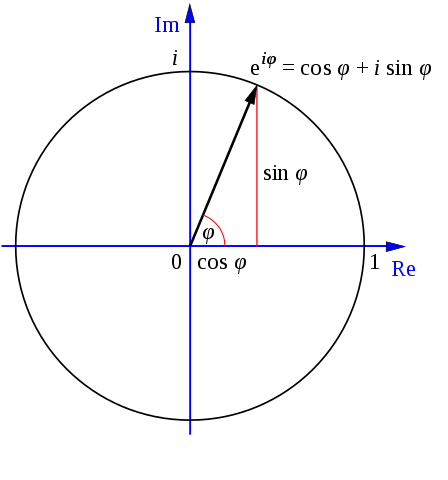
\includegraphics[width=0.5\textwidth]{figures/09.01.png}
\end{center}
There is a special case of this formula known as Euler's identity and regardless of the number of times I prove it to myself, I just can't believe it all works out like this. If $x = \pi$ then
\begin{equation}
	e^{\jmath \pi} = -1
\end{equation}
which has just about every important mathematical thing in it: exponentials, imaginary numbers, constants of the universe, negative numbers, the single unit. In fact, add the one back to the other side and you'll see a zero appear from the depths. All this to say, recognizing the interrelatedness of exponential functions to just about everything else in mathematics and engineering will help us here and elsewhere immensely.


\section{The Laplace transform}
Mathematically, the Laplace transform is simple to describe. First, get yourself a curly L, looks like
this
\begin{equation}
	\mathcal{L}
\end{equation}
Next to that $\mathcal{L}$, put some curly brackets, like so

\begin{equation}
	\mathcal{L}\{\}
\end{equation}
Within those brackets put some function, say one of time, $f(t)$
\begin{equation}
	\mathcal{L}\{f(t)\} = \text{The Laplace transform of } f(t)
\end{equation}

We may also, sometimes, take a function's name, say $f(t)$, capitalize it, $F(t)$, and call that the Laplace transform. I am not personally the biggest fan of this notation as it can become quite distracting and confounding when combined with other transforms you might want to one day use, such as Fourier transforms, Hilbert transforms, and so on. 

I prefer to designate my Laplace transforms with a squiggly sign over a capitalized version of the function name, like so

\begin{equation}
	\mathcal{L}\{f(t)\} = \tilde{F}(s)
\end{equation}
That squiggly line, and many of those that follow, help explain what the Laplace transform is kind of doing to the reality around you. It's seeing relationships outside of time, cast in a plane of infinite exponential sine waves, with bottomless zeros and infinities you can draw a small circle around. The Laplace transform, should be, I believe, a transformative way of viewing the world around you. The power of the Laplace transform (and its ilk) is to reveal useful realities to us and our machines. Turns out there's more to life than just the time ahead of us. And we can usefully describe it. 

Some of those astute among you will notice I tried to slip something by you in the above definition. (Those of you glancing over the mathematics, get yourself back in the habit of $reading$ mathematics, out loud if need be. Make sure you understand what I'm saying before agreeing to it.) What I tried to sneak into this definition is a new variable $s$ that somehow our function, $f(t)$, became in terms of when transformed. We will get into the more mystical nature of the $s$-plane and its variable $s$, but for now, let's just call it some dummy variable. To you, at this point, it is just some stranger you've met in the street. You don't know them at all. First thing you've got to do, is say, Hello.

Before any of that, though, we must get to the definition of the definition of the Laplace transform. It is what we do to a function $f(t)$ to yield another equation $\tilde{F}(s)$. In that sense, the Laplace transform is defined as

\begin{equation}
	\mathcal{L}\{f(t)\} = \int_0^{\infty}e^{-st}f(t)dt
\end{equation}
which is to say it is the integral over all of time of the product of our function $f(t)$ with an exponential function raised to a power of time, $t$, scaled negatively with some dummy variable, $s$. Essentially, if I were to multiple my function, $f(t)$ at every point in time with a probing function $e^{-st}$ and summed it all up, what would I get? And more importantly to all of this, what would it tell me?

Another way of thinking about what the Laplace transform is ``doing'' is to think about what the mathematics itself is proposing to do. It's taking some function, $f(t)$, and wrapping it along a real and an imaginary exponential, producing both sines and cosines.

\section{The Laplace transform of 1}
Let me start off with the simplest number I can think of, sophist that I am. What is the Laplace transform of the number 1. If I can't solve this integral for the number 1, what the heck can I do? So let's convince ourselves that we can solve at least that much.

\begin{equation}
	\mathcal{L}\{f(t)\} = \mathcal{L}\{(1)\} = \int_0^{\infty}e^{-st}(1)dt
\end{equation}

Some, at this point, might be concerned with that $\infty$ up there in this integral. It creates what is sometimes called an improper integral, that is, one which has either (or both) limits of infinity or an integrand that approaches infinity at one or more points in the range of integration\footnote{This latter fact forms much of the basis of our understanding of control theory.}. To get around this improperness, we create for ourselves yet another dummy variable, let's call this one $A$. Thus we can also write the Laplace transform as

\begin{equation}
	\mathcal{L}\{(1)\} = \int_0^{\infty}e^{-st}(1)dt = \lim_{A\rightarrow \infty}\int_0^{A}e^{-st}(1)dt 
\end{equation}
which is the integral from $0$ to $A$ -- which we can do -- evaluated, ultimately, as $A$ goes infinitely. We take the antiderivative, bounded by our limits, to be
\begin{align}
	\lim_{A\rightarrow \infty}\int_0^{A}e^{-st}(1)dt &= \lim_{A\rightarrow \infty}\left[-\frac{1}{s}e^{-st}\right]_0^A \\
	&= \lim_{A\rightarrow \infty}\left[\left(-\frac{1}{s}e^{-sA}\right)-\left(-\frac{1}{s}\right)\right] \\
	&= \lim_{A\rightarrow \infty}\left[-\frac{1}{s}e^{-sA}+\frac{1}{s}\right]
\end{align}
Let us think about what our limit does. In this case the only factor with an $A$ involved is $-\frac{1}{s}e^{-sA}$. Here, if $A$ becomes huge, it knocks against that $s$, getting even bigger, and knocks against that negative sign to become very very negative. Having a very very negative negative number in our exponential function causes it to go screaming down to 0. In this case, the case where the function $f(t) = 1$, upper infinite limit has obliterated the term associated with it, whereas the lower limit has preserved the term associated with it. This leaves us with the final result:

\begin{equation}
	\mathcal{L}\{f(t)\} = \frac{1}{s}
\end{equation}

\section{The $s$-plane}
Where some see time, others see cycles, decay. The $s$-plane allows us to describe the physical world around us and much of the activity that occurs therein as a bunch of sines and exponentials, which is a quite clever way of squinting at a world that's always got us looking across time. Instead of charting a function or describing some behavior (perhaps of some system) as an amplitude changing over time, let us consider what such a function might look like if on one axis we had a variable describing how fast it decays over time and on the other axis we described how hard the system rattles at each frequency. In plotting such a function, one could see how a system will react under a myriad of conditions which you literally do not have the time to do if you confine yourself to just this slice of reality.

And so we must turn orthogonally to the only world we've ever known and stare into the $s$-domain.

We can start by taking a peak at our variable, $s$. For our first use of the Laplace transform, we didn't even need to know what $s$ was to work with it and to get an answer (of some sort). Indeed I took to calling it a dummy variable since the mechanical evaluation of the mathematics does not require it. It is important to make sure you can always do the math if you are ever called upon to do so. For much of what follows clear and clever shorthand will help us to view signals in a multitude of ways, including our bundling up of terms within $s$. As with much in life and in this class, $s$ comprises a real component, $\sigma$ and an imaginary component, $\omega$:
\begin{equation}
	s = \sigma + \jmath \omega 
\end{equation}
By themselves these two parameters are underwhelming. When raised as the exponent to an exponential and they start to describe a whole other world. Whether it has been stressed to you in your differential equations class or not, every single differential equation in the world has as at least one of its solutions the combination of exponential functions with and sine (or cosine) waves. The reasons for this range from the philosophic (we are trapped between repetition and degradation) to the mechanical (the derivatives of exponentials and sines and just scaled exponentials and sines). Let us take a look at the form $s$ takes itself for the Laplace transform:
\begin{equation}
	e^{-st} = e^{-(\sigma + \jmath \omega)t} 
\end{equation}
If were were to expand it out, we could perhaps convince ourselves that two separate yet equally important components emerge. One describes a function which dampens a response with time and one which oscillates back and forth with time.
\begin{equation}
	e^{-(\sigma + \jmath \omega)t}= \underbrace{e^{-\sigma t}}_{\text{damping}} + \underbrace{e^{-\jmath \omega t}}_{\text{sinusoids}}
\end{equation} 

The first of these behaviors we can probably prove to ourselves by inspection. If $s >0$, and let us say that it is, then as $t$ gets really large, the exponential function will die down to zero, under the influence of that negative infinity. Therefore, we are right to call $e^{-\sigma t}$ a damping term, since it will eventually smooth everything away to nothingness.

The second of these behaviors requires a brief detour back to our Eulerian days\footnote{One should get use to thinking in both Eulerian and Laplacian terms.}.

A benefit to this whole situation is that it reduces the mathematical complexity of the reality of the situation (represented by the mathematical operation of convolution, which we will get to in a couple weeks) to algebra. 


\section{The linearity of the Laplace transform}
The Laplace transform has at least one property that we must address here, its linearity. As the transform satisfies the two conditions of linearity previously established, homogeneity (a response is proportional to an excitation) and additivity (a response is the sum of excitations), we can use it with near reckless abandon for linear systems, i.e., those we will concern ourselves with here.

The linearity of the transform means that the transform of a sum is that same as the sum of individual transforms. Moreover, scaling constants are not affected by the transform and remain constant throughout. Mathematically this may all be stated as:
\begin{equation}
	\mathcal{L}\{a_1f_1(t) + a_2f_2(t)\} = a_1\tilde{F}_1(s) + a_2\tilde{F}_2(s)
\end{equation}
This result is convenient for more involved analyses and is one we must keep in mind.

\section{The Laplace transform of $e^{at}$}
To apply the Laplace transform, we take our $f(t)$, multiple it by our probing function, $e^{-st}$, and integrate over all time (for the moment, let us stipulate $s > a$):
\begin{align}
	\tilde{F}(s) = \mathcal{L}\{f(t)\} &= \int_0^{\infty}e^{-st}e^{at} dt \\
	&= \int_0^{\infty}e^{(a-s)t} dt \\
	&= \int_0^{\infty}e^{-(s-a)t} dt \\
	&= \left[-\frac{e^{-(s-a)t}}{s-a}\right]_0^{\infty} \\
	&= \left(-\frac{e^{-(s-a)\infty}}{s-a}\right) - \left(-\frac{e^0}{s-a}\right) \\
	&= 0 + \frac{1}{s-a} \\
	\mathcal{L}\{e^{at}\} &= \frac{1}{s-a}
\end{align}
From this we can perhaps see a pattern or two. Our Laplace transform took the exponent of the exponential and dropped it down in the denominator with $s$ as a subtractive component. Thus, one might just as well commit to memory that that Laplace transform of $e^{4t}$ is $\frac{1}{s - 4}$ as look it up in a table. From this simple derivation we now know that $e^{-0.25t}$ transforms to $\frac{1}{4s + 1}$ and could even convince ourselves that $3e^{-2t}$ becomes $\frac{3}{s+2}$. In fact, hopefully we can recognize that our previous derivation of the Laplace transform of the number 1 is just the case where $a = 0$ when $f(t) = e^{at}$.

You might wonder, what do I care about having a new fraction? What good does that do me? Already it has told you something you likely didn't know: as the values of $a$ and $s$ approach equality, the fraction blows up to infinity. We have what we call a ``pole'' at $s = a$.

\section{The Laplace transform of $dx/dt$}
Generally one does not spend a lot of time working through the mathematical conjuring of taking the Laplace of a derivative. The reason for this is because its final form is easy to learn, memorize, and deploy readily. 

Let us begin with a simple, perhaps much too simple, example.

\begin{equation}
	\frac{dx}{dt} - ax = 0
\end{equation}
Leveraging what we've learned of the linearity of our technique, let's find the Laplace transforms each portion of that equation. 

\begin{align}
	\text{Laplace transform 1 } &= \int_{0}^{\infty} e^{-st}\frac{dx}{dt} dt \\
	\text{Laplace transform 2 } &= \int_{0}^{\infty} e^{-st} x dt
\end{align}
The latter equation, ``Laplace transform 2'' is just another way of saying $\mathcal{L}\{x(t)\}$, so we can feel comfortable simply labeling that as $\tilde{X}(s)$.

The former equation requires us to integrate by parts. I will be assumed here that some calculus teacher somewhere once taught you the importance of integration by parts. It will be further assumed here that you know how to do it or could figure out how to do it if called upon to do so. As such, I will not belabor its implementation here and instead present my formulation of the logic of the situation for you to follow:
\begin{align}
	\mathcal{L}\left\{\frac{dx}{dt}\right\} &= \int_{0}^{\infty} e^{-st}\frac{dx}{dt} dt \\ 
	&= -\int_{0}^{\infty} x(t)\left(-se^{-st}dt\right) + \left[xe^{-st}\right]_0^{\infty} \\
	&= s\int_{0}^{\infty} x(t)\left(e^{-st}dt\right) + \left[\left(xe^{-\infty}\right) - \left(xe^{0}\right) \right]\\
	&= s\tilde{X}(s) - x(0)
\end{align}
What this end result suggests to us, is that the Laplace of the derivative of some function $x(t)$ is the Laplace of the function itself, $\tilde{X}(s)$, multiplied by $s$ to which an initial condition, $x(0)$ is subtracted.

Combining these two results and rewriting:

\begin{align}
	\mathcal{L}\left\{\frac{dx}{dt} - ax = 0\right\} \rightarrow \mathcal{L}\left\{\frac{dx}{dt}\right\} - \mathcal{L}\left\{ax\right\} &= \mathcal{L}\left\{0\right\} \\
	s\tilde{X}(s) - x(0) - a\tilde{X}(s) &= 0 \\
	\tilde{X}(s)\left(s - a\right) &= x(0) \\
	\tilde{X}(s) &= \frac{x(0)}{s - a}
\end{align}
Without too much squinting, we can probably see that such a form is quite close to what we found for our exponential function's transformation, $\frac{1}{s - a}$. In fact, as will become clearer and more comfortable to you over time, is that indeed we can begin to quickly map a solution to a differential equation by first transforming it over the $s$-domain. In this particular case, we can hazard a guess that a solution to the differential equation $\frac{dx}{dt} -ax = 0$ is the function $x(t) = x(0)e^{at}$, which indeed from inspection appears to work.

It you didn't catch it there, let me point it out here: you have just learned a very neat mathematical trick for an engineer. This might be the quickest way to solve a differential equation that you will ever know of. 

We've taken a differential equation and reduced it to simple algebra.

\section{The Laplace transform in RLC circuits}
\subsection{Resistors}
To find the voltage drop across a resistor we apply Ohm's law, $v = iR$. To go from the time-domain to the Laplace-domain for is notationally simple:
\begin{align}
	v(t) & \rightarrow \tilde{V}(s) \\
	i(t) & \rightarrow \tilde{I}(s) \\
	v(t) = i(t)R & \rightarrow \tilde{V}(s) = \tilde{I}(s)R
\end{align}
That is, the voltage drop in the $s$-domain is equal to the current in the $s$-domain, scaled to the resistance, $R$.


\subsection{Inductors}
\begin{align}
	v(t) & \rightarrow \tilde{V}(s) \\
	i(t) & \rightarrow \tilde{I}(s) \\
	v(t) &= L\frac{di(t)}{dt} 
\end{align}
Recall from a previous section that the Laplace of a derivative, $\mathcal{L}\{\frac{dx}{dt}\}$ is equal to the product of the Laplace of the original function and $s$ (with the initial conditions subtracted): $s\tilde{X}(s) - x(0)$. We can apply this same logic to solve the above problem, yielding the inductor's behavior:
\begin{align}
	v(t) &= L\frac{di(t)}{dt} \\
	\tilde{V}(s) &= L(s\tilde{I}(s) - i(0)) \\
	\tilde{V}(s) &= sL\tilde{I}(s) - Li(0)
\end{align}

We can even redraw the circuit to see it as we would from the $s$-domain. If I've got a circuit, that starts with a horizontal wire with a current $\tilde{I}(s)$ going through it, I've currently got a potential of $\tilde{V}(s)$ at the rightmost end of that wire. Connecting that wire vertically, we can walk across our equation and see what it's telling us. Our first element is going to affect the current by $sL\tilde{I}(s)$. That's our inductor. We continue our KVL-inspired walk and see that we have a negative drop (a rise) in potential equal to $Li(0)$, the current at our initial condition scaled to our inductor's size. This is a potential source. From this, we have a new vantage point to survey circuits from. Where before we thought of voltage sources as blackboxes, there's a curious response that gets induced in them.

If we were to solve for $\tilde{I}(s)$ by rearranging the equation
\begin{equation}
	\tilde{I}(s) = \frac{\tilde{V}(s)}{sL} + \frac{i(0)}{s}
\end{equation}
and we can redraw this as a parallel circuit. Or essentially, we are losing $\tilde{I}(s)$ through a node with two branches (see the two components on the right hand side). So for our rightmost branch we have a current source, scaled to $1/s$, and then we have our inductor, with an inductance of $sL$.

This technique is extensible to other electronic components. And is in fact another way of transforming our circuits, should the need or desire arise, more specifically source transformation with voltage sources in series with an inductor and current source in parallel with an inductor.

\subsection{Capacitors}

Imagine you've got current going into a capacitor and it's forming a potential on either side of it. we can describe this as 
\begin{equation}
	i = C\frac{dv}{dt}
\end{equation}
We can take the Laplace of both sides
\begin{align}
	\mathcal{L}\{i\} &= \mathcal{L}\{C\frac{dv}{dt}\} \\ 
	\tilde{I}(s) &= C(s\tilde{V}(s) - v(0)) \\
	\tilde{I}(s) &= Cs\tilde{V}(s) - Cv(0)
\end{align}
which is to say we have a current, $\tilde{I}(s)$, being divvied up at a node between two branches. The rightmost branch is a source, $v(0)$, scaled by a capacitance, $C$. (And because it's negative, it turns out this branch is actually entering the node just like $\tilde{I}(s)$). The other branch is a capacitor, $1/C$, multiplied by $s$. 

Just as before with the inductor we can also imagine transforming this source. The simplest way I can think to prove that to ourselves is to rearrange our equation
\begin{equation}
	\tilde{V}(s) = \frac{1}{sC}\tilde{I}(s) + \frac{v(0)}{s}
\end{equation}
From this we can see that our potential drop across a series connected components, $\tilde{V}(s)$ is first dropped by a capacitor $1/sC$, and then dropped by a source, $v(0)$ scaled to $s$.

\begin{equation}
	v(t) = \frac{1}{C}\int_{t_1}^{t_2}
\end{equation}

\subsection{RLC circuits}
Combining these results and recognizing the linearity of each, in a series RLC circuit, we can merely add these all up to yield:
\begin{equation}
	Ri(t) + L\frac{di}{dt} + \frac{1}{C}\int_{-\infty}^{\tau = t}i(\tau)d\tau = v(t)
\end{equation}

\subsubsection{An example}
What is the Laplace transform of a series RLC circuit with $L$ = 1, $R$ = 7, and $C$ = 10.

\section{The general form of just about all systems}
Most systems on earth and else can be expressed by a generalized second-order equation 
\begin{equation}s^2 + 2\zeta\omega_n s  + \omega_n^2\end{equation} 
where $\zeta$ is the damping coefficient and $\omega_n$ is the natural frequency of the system.
\begin{itemize}
	\item \textbf{The natural frequency} is the frequency at which a system tends to oscillate in the absence of any driving or damping forces. It's just what wants to happen.
	\item \textbf{The damping coefficient}, or the damping ratio, is a dimensionless measure of decay. It describes how oscillations in a system die down after a disturbance.
\end{itemize}


\subsection{Undamped systems}
When $\zeta = 0$, a system comprises a single harmonic oscillator, as is the case of a mass suspended by a perfect spring. This is what we would expect with no ``real'' components ($e^{\jmath \omega_n t}$) 
\begin{itemize}
	\item Two imaginary poles at $\pm \jmath \omega_n$
	\item Undamped sinusoid with frequency equal to the imaginary part of the pole. 
	\item Solution: $f(t) = A\cos (\omega_n t - \phi)$
\end{itemize}

\subsection{Underdamped systems}
When $0< \zeta < 1$, a system  will initially oscillate in response to a disturbance before dying down to zero. Can be described by the function $e^{\jmath\omega_n\sqrt{1-\zeta^2}t}$ 

\begin{itemize}
	\item Two complex poles at $-\sigma \pm \jmath \omega_d$ 
	\item Damped sinuosoid with exponential envelope. Time constant is equal to the reciprocal of the pole's real part. 
	\item Solution: $f(t) = Ae^{-\sigma t}\cos (\omega t - \phi)$
\end{itemize} 

\subsection{Critically damped systems}
When $\zeta = 1$, a system  decays away as fast as possible with no oscillations or ``overshoots''. As you might expect, this is a desirable outcome for many many cases of engineering design (e.g., the rate at which a door opens or closes) 
\begin{itemize}
	\item Two real poles at $-\sigma$. 
	\item Response: the sum of two scaled exponentials of the same time constant, one scaled to time. 
	\item Solution: $f(t) = k_1e^{-\sigma t} + k_2te^{-\sigma t}$
\end{itemize}

\subsection{Overdamped systems}
When $\zeta > 1$, a system in does not oscillate and decays  at a slower rate than the critical case. 
\begin{itemize}
	\item Two real poles at $-\sigma_1$ and $-\sigma_2$. 
	\item Response: sum of two exponentials with different time constant
	\item Solution: $f(t) = k_1e^{-\sigma_1 t} + k_2 e^{-\sigma_2 t}$
\end{itemize}



\chapter{The Laplace Transform: II. How to use it}
\section{Two important places, zeros and poles}
\section{``Inverting'' the Laplace transform}
\section{The Laplace transform of $\sin$}
\section{The Laplace transform of $t^n$}
\section{Some applicability}



\chapter{Circuits as ODEs: I. First-order}
02/21/2019 – Lecture 12. 
\section{Source-free RC circuits}
\subsection{One resistor, one capacitor}
\subsection{Two or more resistors and/or capacitors}
\section{Source-free ``active'' circuits}
\section{First-order systems with sources}
\section{Several singular functions}
\subsection{Unit step function, $u(t-t_0) = 1, t>t_0$}
\subsubsection{The Laplace transform of the unit step function}
\subsection{Unit impulse function, $\delta(t) = du(t)/dt$}
\subsubsection{Its ``sifting'' abilities}
\subsubsection{The Laplace transform of the unit impulse function}
\subsection{Unit ramp function, $r(t) = \int u(t)dt $}
\subsubsection{The Laplace transform of the unit impulse function}



\chapter{Circuits as ODEs: II. Second-order}
02/26/2019 – Lecture 13. 
\section{A series RLC circuit}



\chapter{System response: I. Convolution; Homework III}
02/28/2019 – Lecture 14. 
\section{An introduction to thinking in systems}
Viewing everything as a ``system''. 
\subsection{Domains of interest, of command}
\subsection{The time-domain, or: our typical realm}
\subsection{The frequency-domain, or: our new realm}
\subsection{The $s$-domain, or: our magical realm}
\section{Inputs and outputs}
\section{Somewhere in the between}
\section{Convolution in the time-domain}
\section{Multiplication in the frequency- and $s$-domain}



\chapter{System response: II. Stability}
03/12/2019 – Lecture 15. 
\section{An introduction}
\subsection{What do we mean by stability?}
\section{Undamped, $\zeta = 0$}
\section{Underdamped, $0 < \zeta < 1$}
\section{Overdamped, $\zeta > 1$}



\part{\& Signals}



\chapter{System response: III. The frequency domain}
03/14/2019 – Lecture 16. 



\chapter{System response: IV. Filters}
03/19/2019 – Lecture 17. 



\chapter{System response: V. Feedback; Homework IV}
03/21/2019 – Lecture 18. 



\chapter*{Exam II}
03/26/2019



\part{in Biomedical Engineering}



\chapter{Bioelectricity: I. Passive properties}
03/28/2019 – Lecture 19. 
\section{Modeling biological material with a simple circuit, $R_1 + (R_2||C)$}
\section{Resistance-Reactance Plane}
\section{What can we do with this information?}



\chapter{Bioelectricity: II. Active properties}
04/02/2019 – Lecture 20. 



\chapter{Bioelectricity: III. Measurement}
04/04/2019 – Lecture 21. 



\chapter{Digital circuits: I. Discretization}
04/09/2019 – Lecture 22. 



\chapter{Digital circuits: II. Logic; Homework V}
04/11/2019 – Lecture 23. 



\chapter{Happenstance: A few BME specific situations}
04/16/2019 – Lecture 24. 



\chapter{Circumstance: A few BME specific standards}
04/18/2019 – Lecture 25. 



\chapter{A philosophy of circuits, systems, and signals; Homework VI}
04/23/2019 – Lecture 26. 



\chapter*{Exam III}
04/26/2019 


\part{Assignments}
\chapter*{Homework I}
Assigned January 22, 2019. Due January 31, 2019 as \textit{both} a hard copy in class and a pdf on Canvas.
\setcounter{chapter}{1}
\setcounter{section}{0}
\section{Problem 1}
(15 points)	A typical automated external defibrillator (AED) delivers 200-1000 V in less than 10 ms. 
\begin{enumerate}
	\item If the AED in front us delivers a pulse of 600 V, how much current is needed to deliver 120, 240, and 360 Joules?
	\item Assuming two human hands have a mass of approximately 1 kg, how many chest compressions would be needed to deliver an equivalent amount of energy if each compression had a depth of 5 cm and was delivered at a constant speed of 0.5 m/s every 2 seconds?
	\item If you had the option of having your heart “jump-started” would you choose an AED or the bare hands of a stranger? Justify your answer.
\end{enumerate}

\newpage

\section{Problem 2}
(5 points) A  3.3 V battery you are considering for a wearable you are designing has a total charge of 300 mAh. How many joules is this battery capable of delivering?

\section{Problem 3}
(5 points) A fellow engineer bought a 12 V battery rated for 60 Ah. The experiment you both have in mind will draw 2 A over a 1 k$\Omega$ load. How long can your experiment last?

\section{Problem 4}
(5 points) A piece of medical equipment supplies 135 W at 220 V. How much electrical charge flows through the device in the 10 hours a nurse is on-call using it? And how many electrons does this charge correspond to?


\section{Problem 5}
(10 points) During an in vitro (petri dish) experiment, the peak electric power that a group of stem cells can tolerate without some serious functional consequence is known to have a threshold of about 1 mW. If the power delivered to this group of cells is defined as $p(t) = 2e^{-t}\sin 5t$ [mW], will the cell be harmed and if so how long can power be delivered before the cells are harmed?

\section{Problem 6}
(10 points) Find the equivalent resistances. (Show your work.)
\begin{itemize}
	\item 1 square of resistors (R = 10 k$\Omega$) measured across corners.
	\item 2 resistors (R1 = 10 k$\Omega$, R2 = 4 k$\Omega$) in series.
	\item 3 resistors (R1 = R2 = R3 = 10 k$\Omega$) in parallel.
	\item 4 resistors (R1 = 1 k$\Omega$, R1 = 2 k$\Omega$, R1 = 3 k$\Omega$, R1 = 4 k$\Omega$) in parallel.
	\item 5 resistors (R = 10 k$\Omega$) in a pentagon, measured across each resistor.
\end{itemize}

\section{Problem 7}
(10 points) Hospitals often employ what is known as a dynamic uninterruptible power system (D-UPS) comprising a diesel generator, a synchronous machine, and a kinetic energy unit. By way of example, if the energy to a particular hospital fails, the kinetic energy unit continues to feed 600 kW to the hospital for 20 seconds, allowing the generator and synchronous machine to take over and feed the load.
\begin{enumerate}
	\item What is the total energy capacity of this kinetic energy unit?
	\item If the hospital were operating at 240 kW (instead of the aforementioned 600 kW), how much longer can the unit feed the load?
\end{enumerate}


\section{Problem 8}
(10 points) Current passing through an electrical element in an AC situation can generally be defined as $i(t) = A \sin \omega t$. 
\begin{enumerate}
	\item Determine the energy on this element if the voltage across it is 
\\
$v(t) = B \cos \omega t$.
	\item Plot current, voltage, and energy as functions of time using MATLAB (or an equivalent software package). You may use any values of $A$, $B$, and $\omega$ that you’d like, but unit values (=1) might make your life/work easier. (Present the code you used to arrive at your plot.)
\end{enumerate}


\section{Problem 9}
(10 points) The materiality of the human body ensures that it puts up some resistance to the flow of current. Find some values of impedance for the following human body parts. Be sure to cite your source(s) and explain why you trust it. (Given that there is a frequency dependence to these values, you may present any value of impedance found between 1 | 100 kHz.)
\begin{enumerate}
	\item The whole body, from head to toe.
	\item A single limb (such as an arm or a leg).
	\item Blood.
	\item Muscle.
	\item Fat.
\end{enumerate}


\section{Problem 10}
(20 points) For the circuit shown below.
\begin{center}
	\includegraphics{figures/hw1.10.png}
\end{center}

\begin{enumerate}
	\item Use the delta-wye transformation rule to determine the power dissipated by R1.
	\item Find the voltage at node a (just after R1). 
	\item If R4 were changed to 100 $\Omega$, would the results to (10.1) and/or (10.2) change? How do you know?
	\item How many nodes, branches, and loops are there?
	\item What is the voltage at each node, the current through each branch?
\end{enumerate}




\chapter*{Homework II}
Assigned February 8, 2019. Due February 14, 2019 as \textit{both} a hard copy in class and a pdf on Canvas.
\setcounter{chapter}{2}
\setcounter{section}{0}

\section{Problem 1}
Though we rarely think about it, resistors have a directionality to them. To prove this to ourselves, let us consider a rectangular prism with a square cross-sectional area with a width of $a$ on its square face, a length of $L$, and a resistivity of $\rho$. An example of such a conductor may be seen in the figure below.
\begin{center}
	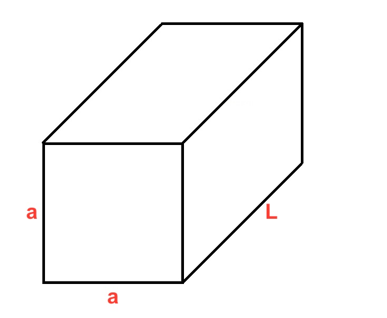
\includegraphics{figures/hw2.01.png}
\end{center}
\begin{enumerate}
	\item Determine the resistance between two parallel square faces, two parallel rectangular faces, and determine the ratio of these two resistances.
	\item How would you go about performing a similar analysis for a resistor with a circular cross-sectional area? 
\end{enumerate}



\section{Problem 2}
For the circuit shown below, find the current flowing though $R3$ ($i3$) and the current flowing through $R4$ ($i4$). 
\begin{center}
	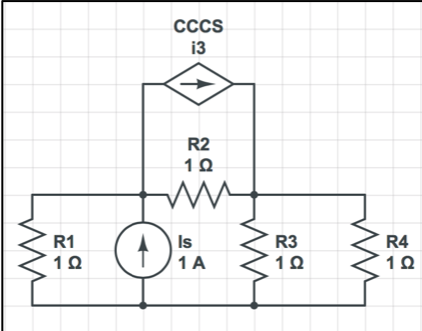
\includegraphics{figures/hw2.02.png}
\end{center}


\section{Problem 3}
For the circuit shown below.
\begin{center}
	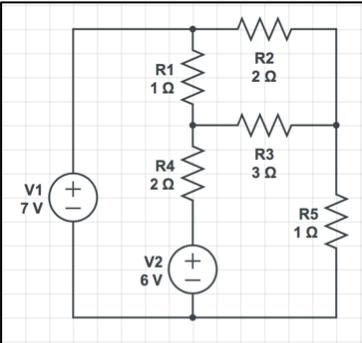
\includegraphics{figures/hw2.03.png}
\end{center}
\begin{enumerate}
	\item Perform a mesh analysis and determine the mesh currents in each loop. (You may solve it any way you’d like, just walk me through how you solve it.)
	\item Determine the current through R3. How you would actually measure the actual current through R3 in an actual circuit?
\end{enumerate}



\section{Problem 4}

For the circuit shown below, determine the Thévenin and Norton equivalent circuits between terminals a and b.
\begin{center}
	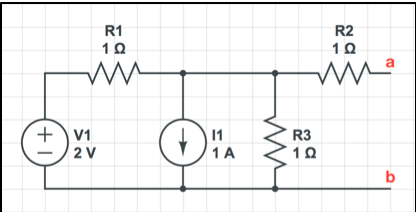
\includegraphics[width=0.5\textwidth]{figures/hw2.04.png}
\end{center}

\section{Problem 5}
Using the superposition theorem, find the voltage \color{red} \textbf{Va} \color{black} in in the circuit shown below. Be sure to show all your steps.

\begin{center}
	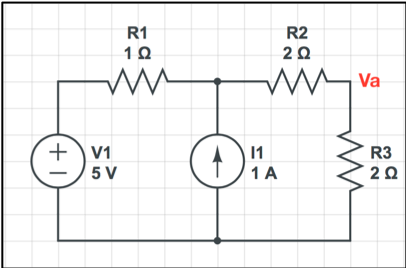
\includegraphics[width=0.5\textwidth]{figures/hw2.05.png}
\end{center}

\section{Problem 6}
For the circuit shown below, determine the Thévenin equivalent circuit that would be found between the \color{red}\textbf{a} \color{black} and \color{red} \textbf{b} \color{black} terminals.
\begin{center}
	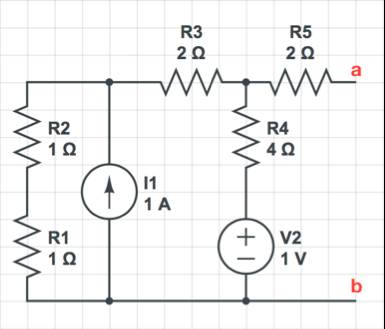
\includegraphics[width=0.5\textwidth]{figures/hw2.06.png}
\end{center}

\section{Problem 7}
Electrocardiographic (ECG) signals tend to be about 1 mV before being measured by a monitoring system (that is, it is about 1 mV just before it gets to our skin). If skin resistance is about 100 k$\Omega$, what is the voltage as measured by our system if our system has an input impedance of 500 k$\Omega$, 1 M$\Omega$, and 2M$\Omega$. You may model the entire situation as a series combination of elements. What effect do you think sweating at the area of measurement will have on the voltages you just calculated?

\section{Problem 8}
For the circuit below, find the current passing through each element.

\begin{center}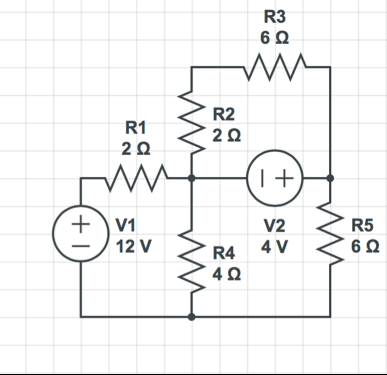
\includegraphics{figures/hw2.08.png}\end{center}

\section{Problem 9}
Our blood vessels are something of glorified hollow conductive cylinders. Let us assume that the resistivity of the vessel, $\rho$, is constant throughout our length of interest, $L$. If we were to apply a potential difference, $V$, between the inner surface of the blood vessel (with radius $a$) and the outer surface of the blood vessel (with radius $b$), what would be the resistance we measure? (Hint: the differential resistance in this case is equal to $dR = \rho(dL/A)$.)

\section{Problem 10}
To the extent you feel comfortable sharing this information, have you ever had to interact with a piece of biomedical equipment that utilized electronic circuitry? (This may include anything from a Fitbit to an ECG and beyond.) If so, what aspects of that experience relating to the equipment did you find fascinating, and which aspects of it would you personally liked to have seen improved? [If you do not wish to share a personal experience or perhaps do not have one to share, consider the question in the abstract: \textit{knowing what you know, what might you wish to see improved regarding current medical instruments}?]


%\setcounter{chapter}{4}


\end{document}